%%%%%%%%%%%%%%%%%%%%%%%%%%%%%%%%%%%%%%%%%
% Masters/Doctoral Thesis 
% LaTeX Template
% Version 1.43 (17/5/14)
%
% This template has been downloaded from:
% http://www.LaTeXTemplates.com
%
% Original authors:
% Steven Gunn 
% http://users.ecs.soton.ac.uk/srg/softwaretools/document/templates/
% and
% Sunil Patel
% http://www.sunilpatel.co.uk/thesis-template/
%
% License:
% CC BY-NC-SA 3.0 (http://creativecommons.org/licenses/by-nc-sa/3.0/)
%
% Note:
% Make sure to edit document variables in the Thesis.cls file
%
%%%%%%%%%%%%%%%%%%%%%%%%%%%%%%%%%%%%%%%%%

%----------------------------------------------------------------------------------------
%	PACKAGES AND OTHER DOCUMENT CONFIGURATIONS
%----------------------------------------------------------------------------------------

\documentclass[11pt, oneside]{Thesis} % The default font size and one-sided printing (no margin offsets)

\graphicspath{{Pictures/}} % Specifies the directory where pictures are stored

\usepackage[square, numbers, comma, sort&compress]{natbib} % Use the natbib reference package - read up on this to edit the reference style; if you want text (e.g. Smith et al., 2012) for the in-text references (instead of numbers), remove 'numbers' 

\usepackage{amsmath} % Mathe
\usepackage{mathtools} % Mathe
\usepackage{amsfonts} % Mathesymbole
\usepackage{calc}
\usepackage{url}
\usepackage{listings}
\usepackage{titlesec}
\usepackage{placeins}
\usepackage{listings}
\usepackage{xcolor}

\titleformat
{\chapter} % command
[display] % shape
{\normalfont\Large\bfseries} % format
{Chapter \ \thechapter}
{0.5ex} % sep
{
    \rule{\textwidth}{1pt}
    \vspace{0ex}
    \centering
} % before-code
[
\vspace{-0.5ex}%
\rule{\textwidth}{0.3pt}
] % after-code

\lstdefinelanguage{scala}{
  morekeywords={abstract,case,catch,class,def,%
    do,else,extends,false,final,finally,%
    for,if,implicit,import,match,mixin,%
    new,null,object,override,package,%
    private,protected,requires,return,sealed,%
    super,this,throw,trait,true,try,%
    type,val,var,while,with,yield,specialized},
  otherkeywords={<-, =>,<\%,<:,>:,\#,@},
  sensitive=true,
  morecomment=[l]{//},
  morecomment=[n]{/*}{*/},
  morestring=[b]",
  morestring=[b]',
  morestring=[b]"""
}

\definecolor{ggray}{gray}{0.5}
\definecolor{Green}{HTML}{005500}
\definecolor{Blue}{HTML}{000099}

\renewcommand{\ttdefault}{pcr}
\lstset{frame=tb,
  language=scala,
  aboveskip=6mm,
  belowskip=0mm,
  showstringspaces=false,
  columns=flexible,
  %basicstyle={\footnotesize \ttfamily},
  basicstyle=\renewcommand{\baselinestretch}{0.95}\ttfamily,%
  %basicstyle=\LSTfont,
  numbers=none,
  numbersep=5pt,
  numberstyle=\tiny\color{Blue},
  keywordstyle=\color{Blue},
  commentstyle=\color{Green},
  frame=single,
  breaklines=true,
  breakatwhitespace=true
  tabsize=3
}


\hypersetup{urlcolor=blue, colorlinks=true} % Colors hyperlinks in blue - change to black if annoying
\title{\ttitle} % Defines the thesis title - don't touch this

\begin{document}

\frontmatter % Use roman page numbering style (i, ii, iii, iv...) for the pre-content pages

\setstretch{1.3} % Line spacing of 1.3

% Define the page headers using the FancyHdr package and set up for one-sided printing
\fancyhead{} % Clears all page headers and footers
\rhead{\thepage} % Sets the right side header to show the page number
\lhead{} % Clears the left side page header

\pagestyle{fancy} % Finally, use the "fancy" page style to implement the FancyHdr headers

\newcommand{\HRule}{\rule{\linewidth}{0.5mm}} % New command to make the lines in the title page

% PDF meta-data
\hypersetup{pdftitle={\ttitle}}
\hypersetup{pdfsubject=\subjectname}
\hypersetup{pdfauthor=\authornames}
\hypersetup{pdfkeywords=\keywordnames}               
            

%----------------------------------------------------------------------------------------
%	TITLE PAGE
%----------------------------------------------------------------------------------------

\begin{titlepage}
\begin{center}

\textsc{\LARGE \univname}\\[1.5cm] % University name
\textsc{\Large Master Thesis}\\[0.5cm] % Thesis type

\HRule \\[0.4cm] % Horizontal line
{\huge \bfseries \ttitle}\\[0.4cm] % Thesis title
\HRule \\[1.5cm] % Horizontal line
 
\begin{minipage}{0.4\textwidth}
\begin{flushleft} \large
\emph{Author:}\\
\href{https://github.com/nicolasstucki/}{\authornames} % Author name - remove the \href bracket to remove the link
\end{flushleft}
\end{minipage}
\begin{minipage}{0.4\textwidth}
\begin{flushright} \large
\emph{Supervisor:} \\
\href{https://github.com/VladUreche}{\supname} % Supervisor name - remove the \href bracket to remove the link  
\end{flushright}
\end{minipage}\\[3cm]
 
\large \textit{A thesis submitted in fulfilment of the requirements\\ for the degree of \degreename}\\[0.3cm] % University requirement text
\textit{in the}\\[0.4cm]
\groupname\\\deptname\\[2cm] % Research group name and department name
 
{\large \today}\\[4cm] % Date
%\includegraphics{Logo} % University/department logo - uncomment to place it
 
\vfill
\end{center}

\end{titlepage}


%----------------------------------------------------------------------------------------
%	ABSTRACT PAGE
%----------------------------------------------------------------------------------------

\addtotoc{Abstract} % Add the "Abstract" page entry to the Contents

\abstract{\addtocontents{toc}{\vspace{1em}} % Add a gap in the Contents, for aesthetics

\color{red}The Thesis Abstract is written here (and usually kept to just this page). The page is kept centered vertically so can expand into the blank space above the title too\ldots\color{black}
}

\clearpage % Start a new page

%----------------------------------------------------------------------------------------
%	ACKNOWLEDGEMENTS
%----------------------------------------------------------------------------------------

%\setstretch{1.3} % Reset the line-spacing to 1.3 for body text (if it has changed)

%\acknowledgements{\addtocontents{toc}{\vspace{1em}} % Add a gap in the Contents, for aesthetics

%The acknowledgements and the people to thank go here, don't forget to include your project advisor\ldots
%}
%\clearpage % Start a new page

%----------------------------------------------------------------------------------------
%	LIST OF CONTENTS/FIGURES/TABLES PAGES
%----------------------------------------------------------------------------------------

\pagestyle{fancy} % The page style headers have been "empty" all this time, now use the "fancy" headers as defined before to bring them back

\lhead{\emph{Contents}} % Set the left side page header to "Contents"
\tableofcontents % Write out the Table of Contents

\lhead{\emph{List of Figures}} % Set the left side page header to "List of Figures"
\listoffigures % Write out the List of Figures

%\lhead{\emph{List of Tables}} % Set the left side page header to "List of Tables"
%\listoftables % Write out the List of Tables

%----------------------------------------------------------------------------------------
%	ABBREVIATIONS
%----------------------------------------------------------------------------------------

\clearpage % Start a new page

\setstretch{1.5} % Set the line spacing to 1.5, this makes the following tables easier to read

\lhead{\emph{Abbreviations}} % Set the left side page header to "Abbreviations"
\listofsymbols{ll} % Include a list of Abbreviations (a table of two columns)
{
\textbf{JVM} & \textbf{J}ava \textbf{V}irtual \textbf{M}achine \\
\textbf{JIT} & \textbf{J}ust \textbf{I}n \textbf{T}ime \\
\textbf{LHS} & \textbf{L}eft \textbf{H}and \textbf{S}ide \\
\textbf{RHS} & \textbf{R}igth \textbf{H}and \textbf{S}ide \\
\textbf{RB} & \textbf{R}adix \textbf{B}alanced \\
\textbf{RRB} & \textbf{R}elaxed \textbf{R}adix \textbf{B}alanced}

%----------------------------------------------------------------------------------------
%	PHYSICAL CONSTANTS/OTHER DEFINITIONS
%----------------------------------------------------------------------------------------

%\clearpage % Start a new page

%\lhead{\emph{Physical Constants}} % Set the left side page header to "Physical Constants"

%\listofconstants{lrcl} % Include a list of Physical Constants (a four column table)
%{
%Speed of Light & $c$ & $=$ & $2.997\ 924\ 58\times10^{8}\ \mbox{ms}^{-\mbox{s}}$ (exact)\\
% Constant Name & Symbol & = & Constant Value (with units) \\
%}

%----------------------------------------------------------------------------------------
%	SYMBOLS
%----------------------------------------------------------------------------------------

%\clearpage % Start a new page

%\lhead{\emph{Symbols}} % Set the left side page header to "Symbols"

%\listofnomenclature{lll} % Include a list of Symbols (a three column table)
%{
%$a$ & distance & m \\
%$P$ & power & W (Js$^{-1}$) \\
% Symbol & Name & Unit \\

%& & \\ % Gap to separate the Roman symbols from the Greek

%$\omega$ & angular frequency & rads$^{-1}$ \\
% Symbol & Name & Unit \\
%}

%----------------------------------------------------------------------------------------
%	DEDICATION
%----------------------------------------------------------------------------------------

%\setstretch{1.3} % Return the line spacing back to 1.3

%\pagestyle{empty} % Page style needs to be empty for this page

%\dedicatory{For/Dedicated to/To my\ldots} % Dedication text

%\addtocontents{toc}{\vspace{2em}} % Add a gap in the Contents, for aesthetics

%----------------------------------------------------------------------------------------
%	THESIS CONTENT - CHAPTERS
%----------------------------------------------------------------------------------------
\mainmatter % Begin numeric (1,2,3...) page numbering

\pagestyle{fancy} % Return the page headers back to the "fancy" style

% Include the chapters of the thesis as separate files from the Chapters folder
% Uncomment the lines as you write the chapters

I% Chapter Template
\pagenumbering{gobble}
\lhead{} 

\chapter{Introduction} % Main chapter title
\pagenumbering{arabic}
\label{Introduction} % Change X to a consecutive number; for referencing this chapter elsewhere, use \ref{ChapterX}

\lhead{\emph{Introduction}} % Change X to a consecutive number; this is for the header on each page - perhaps a shortened title

%----------------------------------------------------------------------------------------
%	SECTION 1
%----------------------------------------------------------------------------------------

\section{Motivation}
With the increase on multicore machines, programs tend to use more parallelism and concurrency. In these contexts, managing mutable data structures introduces more complexity. The managements of the thread safeness can become a burden on the programer and the machine. A simpler approach is using immutable data structures, where the data can't be corrupted and can be accessed directly without any risk. The tradeoffs that must be made are on the creation and modification time of such data structures.

In classical functional programming immutable data structures are a requirement. In languages like Scala where there is a functional side and an object oriented side immutable data is not longer required, but the compiler provides better optimizations on them.

% what are vectors
%% highly optimized
%% lack of efficient concatenation
%%% parallel vector is suboptimal
Scala has a rich collection of immutable data structures as well as parallel versions that divide their work transparently on thread pools. Where the \texttt{Vector} is used as the default general purpose parallel sequence. The immutable vector is designed to have effective constant time in practice on its key operations: get element at index, update element at index, insert on an end of the vector and splitting the vector. But, one of the operations required for parallelism is an efficient concatenation.

% what are rrb tree (RRBTrees paper \cite{RRBTrees})
%% efficient concatenation
%% lacks the other operations
To improve this operation P. Bagwell and T. Rompf proposed a less strict structure for the vector \cite{RRBTrees}. They propose the use of a Relaxed Radix Balanced Tree instead of the current Radix Balanced Tree. With these trees it is additionally possible to implement effective constant time in practice concatenation and inserts in any position. The drawback is in the loss of some optimizations opportunities due to the relaxation.

\section{Objective}
% use rrb-trees for vectors (This project repository \cite{projecRepo})
%% generalize operations
%% without loosing performance other operations
%% keep the optimisations whenever possible
%% implementation aims to be production ready (not prototype)
The main objective of this project was to implement\footnote{Implementation is located a \url{https://github.com/nicolasstucki/scala-rrb-vector} \cite{projecRepo}} version of the Scala immutable Vector using RRB-Trees that could potentially replace the old one. The challenges behind this implementation where to have an implementation that would be as performant as the old one for all operations excepting the concatenation, even when the relaxed representation of the tree can't take advantage of some key optimization. To avoid the complete loss of optimization, ways to apply such optimizations partially where explored and applied.

% benchmark and analysis the performance
%% compare with the current vector
%% compare with other implementation variants
To show and analyse the tradeoffs between the implementations extensive benchmarks where realised on all core operations of the vectors. These compare the current vector with an array of different RRB-Trees including: different tree branching sizes, different implementation of concatenation algorithm and differently unbalanced RRB-Trees. 

\section{Document Structure}
% section 2:
%% 1. introduce the vector and structure of the current vector and the operations in a generic
%% 2. related structures that uses the trees
%% 3. how the tree structure is relaxed and how it affects the operarations
%%% addition of concatenation and insert at
In chapter \ref{VectorStructure} we discuss the data structures and operations: Section \ref{RadixBalancedVectors} describes the current version of the vector structure and operations, section \ref{RelatedStructures} discusses related data structure that use the same trees in other ways (like the iterator of a vector), section \ref{RelaxedRadixBalancedVectors} describes the RRB-Tree and how to relax the operations based on the non relaxed versions.

% section 3: optimizations done on the implementations
%% 1. discussion on representations of data and code. how this affects performance
%% 2. discussion of optimization that aim to amortize the operations to constant time.
%% 3. related structures optimized implementations
In chapter \ref{Optimizations} we describe the optimization done on the current version of the vector and how they are affected by the relaxation. In section \ref{WhereIsTimeSpent} we discuss optimizations on the representation of data and the code. In section \ref{sec:Displays} we describe the optimizations that are used to reduce the algorithmic complexities of some operations. In section \ref{OptimizationRelatedStructures} we describe the implementation of the related structures and optimizations on them.

% section 4: performance in practice
%% 1. Discussion on JVM performance caracteristics and how it was used in the implementation
%% 2-3 How the was performance measured
%% 4 benchmarks results
In chapter \ref{Performance} we discuss the performance of the implementation in practice. In section \ref{InPractice} we describe characteristics of the JVM and how to take advantage of them. In sections \ref{Measuringperformance} and \ref{ImplementationGenerators} we describe how the performance is measured in benchmarks. In section \ref{Benchmarks} we show  the results of the benchmarks and analyse it.

% section 5: testing the correctness of the code
% section 6: related work and future work
% section 7: conclude in section 7
In chapter \ref{Testing} the testing methodology, chapter \ref{RelatedWork} lists the related and future work and finally the conclusion is in chapter \ref{Conclusions}.





I% Chapter Template

\chapter{Immutable Vector Structure and Operations} % Main chapter title

\label{VectorStructure} % Change X to a consecutive number; for referencing this chapter elsewhere, use \ref{ChapterX}

\lhead{\emph{Immutable Vector Structure and Operations}} % Change X to a consecutive number; this is for the header on each page - perhaps a shortened title

%----------------------------------------------------------------------------------------
%	SECTION - Radix Balanced Vectors
%----------------------------------------------------------------------------------------

An immutable vector is an representation for an indexed sequence\footnote{Ordered sequence of elements where each one is identified by its index or position.} of elements with efficient random access and update\footnote{Update in the scene of immutable data structures refers to the creation of a structure with an element changed.}. It also provides operations that allow efficient additions and removal of elements.
 
\section{Radix Balanced Vectors}
\label{RadixBalancedVectors}
% vector as a wrappers for the tree
The current immutable \texttt{Vector} implementation\cite{scalaVector211} of the Scala Collections is a wrapper around an immutable tree. The vector implements its methods based on a set of core efficient operations on the trees.

%-----------------------------------
%	SUBSECTION - Tree structure
%-----------------------------------

\subsection{Tree structure}
\label{RRBTreeStructure}
% describe tree: balancing, filling, block sizes
% hint why radix?
% why structure helps with operations implementation 
The RB-Tree (Relaxed Balanced Tree)  structure is a shallow and densely-filled tree where elements are located only in the leafs and on the left side. The nodes in the tree have a fixed size, whether they're internal nodes, linking to subtrees, or leafs, containing elements. Benchmarks have shown the optimal node size is 32, but as we will later see\footnote{Nodes of size 64 could also be consider, with some trade-offs.}, the node size can be any power of 2, allowing efficient radix-based implementations (see \ref{ComputingIndices}). Figure \ref{badix_balanced} shows this structure for $m$ children on each node. 

\begin{figure}[h!]
  \centering
  \includegraphics[width=\textwidth]{Figures/Radix_Balanced}
  \caption{Radix Balanced Tree Structure}
   \label{badix_balanced}
\end{figure}

The RB-Vector also keeps the height of the tree in the \texttt{depth} field. This height will always be upper bounded by $log_{32}(size-1)+1$ for nodes of 32 branches. Therefore the tree is quite shallow and the complexity to traverse it is considered as effectively constant when taking into account that the size will never be larger than the maximum index representable with \texttt{Int}, which corresponds to a maximum depth of 7 levels\footnote{Maximum depth of $log_{32}(2^{31}) + 1$, which is 6.2.}.

Yet, the tree may have numbers of elements that are not powers of 32. To allow this, the RB-tree fills in the elements in the leafs from the left. The branches on the right that do not contain any element in any of their leafs are not allocated (left as empty references or truncated nodes). For example the tree that would hold 1056 elements in figure \ref{badix_balanced_32} would have empty subtrees on the right of the nodes on the rightmost branch. To prevent out-of-bounds access, the vector has an \texttt{endIndex} field that point to that last index. With this it is possible to have efficient implementations of \texttt{take} and \texttt{append} (see \ref{Operations}), as they make changes on this index rather that the structure of the tree.

\begin{figure}[h!]
  \centering
  \includegraphics[width=0.4\textwidth]{Figures/Radix_Balanced_32}
  \caption{Radix Balanced Tree Structure with nodes of size 32 filled with 1056 elements.}
   \label{badix_balanced_32}
\end{figure}

Similarly, to have efficient implementation of \texttt{drop} and \texttt{prepend} operations (see \ref{Operations}), the vector defines a \texttt{startIndex} field that points to the first element in the tree that is actually used in the vector. In this case, although the leafs are empty on the left of the first element, the nodes are still allocated with the full size. As such, the tree structure is logically still full on the left but elements are never accessed if below the \texttt{startIndex}. An element at some \texttt{index} in the vector will be at \texttt{startIndex + index} in the tree. This allows the balanced radix structure to be maintained regardless of the missing elements on the left. As such, the implementations for \texttt{drop} and \texttt{prepend} will take advantage of the index to avoid restructuring the whole tree.

%-----------------------------------
%	SUBSECTION - Operations
%-----------------------------------
\subsection{Operations}
\label{Operations}
% List core operations
The immutable vector in the current Scala Collections is an indexed sequence, as such it offers a large range of operations. Most of these operations are implemented using a set of core operations that can be implemented efficiently on RB-Trees, those operations are: \texttt{apply}, \texttt{updated}, \texttt{append}, \texttt{prepend}, \texttt{drop} and \texttt{take}. 

% performance log_{32}(n) -> effective constant time
The performances of most operations on RB-Trees have a computational complexity of $O(log_{32}(n))$, equivalent to the height of the tree. This is usually referred as effective constant time because for 32 bit signed indices the height of the tree will bounded by a small constant (see \ref{RRBTreeStructure}). This bound is reasonable to ensure that in practice the operations behave like constant time operations.  
 
% naive implementation just as high level guide
In this section the operations will be presented on a high level\footnote{Ignoring some pieces of code like casts, return types, type covariance, among others.} and without optimization. These reflect the base implementation that is used before adding optimizations, which, in many cases lower the cost of the operations (see Chapter \ref{Optimizations}). This makes the operations in this section act as worst-case scenarios, when none of the optimizations apply and thus the basic operations have to be performed.

For simplicity of code in this section we define:
\begin{lstlisting}[frame=single]
  type Node = Array[AnyRef]
  val Node = Array
\end{lstlisting}


%-----------------------------------
%	SUBSUBSECTION - Apply
%-----------------------------------

\subsubsection{Apply}
\label{sec:apply}
% used in head and last
The \texttt{apply} operation returns the element located at the given index. This is the main element access method and it is used in other methods such as \texttt{head} and \texttt{last}. 

\begin{lstlisting}[frame=single]
def apply(index: Int): A = {
  def getElem(node: Node, depth: Int): A = {
    val indexInNode = // compute index
    if(depth == 1) node(indexInNode)
    else getElem(node(indexInNode), depth-1) 
  }
  getElem(vectorRoot, vectorDepth)
}
\end{lstlisting}

% performance log_{32}(n), hint of displays
The base implementation of the \texttt{apply} operation requires a simple traversal from the root to the leaf containing the element, the path taken is defined by the index of the element and extracted using some efficient bitwise operations (see section \ref{ComputingIndices}). With this traversal of the tree, the complexity of the \texttt{apply} operation is $O(log_{32}(n))$. 

%-----------------------------------
%	SUBSUBSECTION - Updated
%-----------------------------------

\subsubsection{Updated}
\label{sec:updated}
% base implementation needs to update the whole branch
This is the primary operation for transforming the vector. However, since the vector is an immutable data structure, instead of modifying the element in place, this operation returns a new immutable vector and does not modify the existing one. This is the reason it is called \texttt{updated} instead of the more common \texttt{update}.

The updated operation has to recreate the whole branch from the root to the element being updated. The update of the leaf creates a fresh copy of the leaf with the updated element. Then the parent of the leaf also need to create a new node with the updated reference to the new leaf, and so on up to the root. 

\begin{lstlisting}[frame=single]
def updated(index: Int, elem: A) = {
  def updatedNode(node: Node, depth: Int) = {
    val indexInNode = // compute index
    val newNode = copy(node)
    if(depth == 1) {
      newNode(indexInNode) = elem
    } else {
      newNode(indexInNode) = updatedNode(node(indexInNode), depth-1)
    }
    newNode
  }
  new Vector(updatedNode(vectorRoot, vectorDepth), ...)
}
\end{lstlisting}

% with transient states, local updates can be amortised
Therefore the complexity of this operation is $O(log_{32}(n))$, for the traversal and creation of each node in the branch. For example, if some leaf has all it's elements updated from left to right, the branch will be copied as many times as there are updates. We will later explain how this can be optimized by allowing transient states that avoid re-creating the path to the root tree node with each update (see \ref{sec:DisplaysTransient}).
%This operation can be improved to have amortized constant time updates for local updates using displays with transient states. %This way the parent nodes are only updated lazily when absolutely necessary. 
%For example, if some leaf has all it's elements updated from left to right, the leaf will be copied as many times as there are updates, but the parent of that leaf does not change during those operations. 

%-----------------------------------
%	SUBSUBSECTION - Additions
%-----------------------------------

\subsubsection{Append}
% base implementation needs to update the whole branch
The \texttt{appended} operation  (or \texttt{:+}) adds an element to the end of the vector. Its implementation has two cases, depending on the current state of the RB-Tree: If the last leaf is not full the element is inserted at the end of it and all nodes of the last branch are copied. If the leaf is full we must find the lowest node in the last branch where there is sill room left for a new branch. Then a new branch is appended to it, down to the new leaf with the element being appended. 

In both cases the new \texttt{Vector} object will have the end index increased by one. When the root is full, the depth of the vector will also increase by one.

\begin{lstlisting}[frame=single]
def :+(elem: A): Vector[A] = {
  def appended(node: Node, depth: Int): Node = {
    if (depth == 1) 
      copyLeafAndAppend(node, elem)
    else if (!isTreeFull(node.last, depth-1)) 
      copyAndUpdateLast(node, appended(node.last, depth-1))
    else
      copyBranchAndAppend(node, newBranch(depth-1))
  }
  def createNewBranch(depth: Int): Node = {
    if (depth == 1) Node(elem)
    else Node(newBranch(depth-1))
  }
  if(!isTreeFull(root, depth))) 
    new Vector(appended(root, depth), depth, ...)
  else 
    new Vector(Node(root, newBranch(depth)), depth+1, ...)
}
\end{lstlisting}

In the code above, the \texttt{isTreeFull} operation computes the answer using efficient bitwise operations on the end index of the vector.

% performance log_32(n), hint of transient to amortize consecutive appends are amortized 
Due to the update of all nodes in the last branch, the complexity of this operation is $O(log_{32}(n))$. Like the updated operation, append can be optimized by keeping transient states of the immutable vector (see Section \ref{sec:DisplaysTransient}).

\subsubsection{Prepend}
% base implementation needs to update the whole branch
The key to be able to prepend  elements to the tree is the \texttt{startIndex} that the vector keeps in its fields. Without this it would be impossible to prepend an element to the vector without a full copy of the vector to rebalance the RB-Tree. The operation can be split into to cases depending on the value of the start index.

% shift top and start index
The first case is to prepend an element on a vector that start at index 0. If the root is full, create a new root on top with the old root as branch at index 1. If there is still space in the root, shift branches in the root by one to the right. In both sub\-cases, create a new branch containing nodes of size 32, but with only the last branch assigned. Put the element in the last position of this newly created branch and set the start index of the vector to that index in the tree.

The second case is to prepend an element on a vector that has a non zero start index. To do so, we follow the branch of the start index minus one from the root of the tree. If we reaches the a leaf, prepend the element to that leaf. If we encounters an inexistent branch, create it by putting the element in its rightmost position and leaving the rest empty. In both sub\-cases update the parent nodes up to the root.

The new \texttt{Vector} object will have an updated start index and end index, to account for the changes in the structure of the tree. It may also have to increase the depth of the vector if the start index was previously zero. 

\begin{lstlisting}[frame=single]
def +:(elem: A): Vector[A] = {
  def prepended(node: Node, depth: Int) = {
    val indexInNode = // compute index
    if (depth == 1) 
      copyAndUpdate(node, indexInNode, elem)
    else 
      copyAndUpdate(node, indexInNode, 
                prepended(node(indexInNode), depth-1))
  }
  def newBranch(depth: Int): Node = {
    val newNode = Node.ofDim(32)
    newNode(31) = if (depth == 1) elem else newBranch(depth-1)
    newNode
  }
  if (startIndex==0) {
    new Vector(Node(newBranch(depth), root), depth+1, ...)
  } else {
    new Vector(prepended(root, depth), depth, ...)  
  }
}
\end{lstlisting}

% performance log_32(n), hint of transient to amortize consecutive prepends are amortised
Since the algorithm traverses and creates new nodes from the root to a leaf, the complexity of the prepend operation is $O(log_{32}(n))$. Like the updated and appended operations, \texttt{prepended} can be optimized by keeping transient states of the immutable vector (see Section \ref{sec:DisplaysTransient}).


\subsubsection{Concatenation}
% describe high level implementation in vector
Given that elements in an RB-Tree are densely packed, implementations for concatenation and insert will need to rebalance elements to make them again densely packed. In the case of concatenation there are three options to join the two vectors: append all elements of the RHS vector to the LHS vector, prepend all elements from the LHS vector to the RHS vector or simply reconstruct a new vector using a builder. The append and prepend options are used when on of the vectors is small enough in relation to the other one. When vectors become large, the best option is building a new vector, since this avoids creating one instance of the vector each time an element is added.

% performance O(n)
The computational complexity of the concatenation operation on RB-Trees for vectors lengths $n1$ and $n2$ is $O(n1 + n2)$ in general. In the special case where $n1$ or $n2$ is small enough the complexity becomes $O(min(n1,n2)*log_{32}(n1+n2))$, the complexity of repeatedly appending or prepending an element.
%-----------------------------------
%	SUBSUBSECTION - Splits
%-----------------------------------

\subsubsection{Splits}
% used in tail, init, take, takeRight, drop, dropRight
The core operations to remove elements in a vector are the \texttt{take} and \texttt{drop} methods. They are used to implement may other operations like \texttt{splitAt}, \texttt{tail}, \texttt{init}, ...

% describe implementation in vector
Take and drop have a similar implementation. The first step is traversing the tree the leaf where the cut will be done. Then the branch is copied and cleared on one side. The tree may become shallower during this operation, in which case some of the nodes on the top will not be copied and just dropped. Finally, the \texttt{startIndex} and \texttt{endIndex} are adjusted according to the changes on the tree.

% performance log_32(n) 
The computational complexity of any split operation is $O(log_{32}(n))$ due to the traversal and copy of nodes on the branch where the cut index is located. $O(log_{32}(n))$ for the traversal of the branch and then $O(log_{32}(m))$ for the creation of the new branch, where $m$ is the size of the new vector (with $0\leq m \leq n$).


%----------------------------------------------------------------------------------------
%	SECTION - Parallel Vectors
%----------------------------------------------------------------------------------------
\clearpage
\section{Related Structures}
\label{RelatedStructures}

\subsection{Vector Builder}
A vector builder is a special wrapper for a RB-Tree that has an efficient \texttt{append} operation. It encapsulates mutable trees during the building of the vector and then freezes them on the creation of the result. Details of this structures are discussed in section \ref{builder}.

\subsection{Vector Iterator}
A vector iterator is a structure that implements an efficient traversal of the vector. In the case of vectors, it is achieved by direct inorder traversal on trees. Details of this structures are discussed in section \ref{iterator}.

\subsection{Parallel Vectors}
% how are they paralellized (wraps an vector)
% fork-join pool
The parallel vector (or \texttt{ParVector} \cite{scalaParVector211}) is a wrapper around the normal \texttt{Vector} object that uses the parallel collections API instead of the normal collections API. With this, operations on collections get executed transparently on fork-join thread pools rather that on the main thread. In order to execute in parallel, the parallel vector needs to be split into chunks, that are processed in parallel and later combined. This is where the \texttt{Splitter} and \texttt{Combiner} objects come into play.


% why do they suffer performance wise (no efficient concat)
The use of a vector combiner produces additional overhead, since requires an concatenation of vector. To reduce this excessive overhead on concatenation the current implementation does it lazily by buffering vectors. Once all the vectors are computed a new one is build by traversing all the vectors in the buffer. 

%-----------------------------------
%	SUBSUBSECTION - Splitter
%-----------------------------------

\paragraph{Splitter (Iterator)}
% split into half 
To divide the work into tasks for the thread pool, a splitter is used to iterate over all elements of the collection. Splitters are a special kind of iterator that can be split at any time into some partition of the remaining elements. In the case of sequences the splitter should retain the original order. The most common implementation consists in dividing the remaining elements into two half. 

The current implementation of the immutable parallel  vector uses the common division into 2 parts of same size. The drop and take operations are used divide the vector for the two new splitters.

%-----------------------------------
%	SUBSUBSECTION - Combiner
%-----------------------------------

\paragraph{Combiner (Builder)}
% lazy combiner
Combiners are used to merge the results from different tasks (in methods like map, filter, collect, ...) into the new collection. Combiners are a special kind of builder that is able to merge to partial results efficiently. When it's impossible to implement efficient combination operation, usually a lazy combiner is used. The lazy combiner keeps all the sub-combiners in an array buffer and only when the end result is needed they are combined by building a new vector with all elements in the vectors contained in the buffer. This alternative comes with a drawback on loss of parallelism of the vector building at the end of the combination as this is done in a single thread. 

The current implementation of the immutable parallel vector uses the lazy approach because of its inefficient concatenation operation. One of the consequences of this is that the parallel operations will always be bounded by this sequential building of a vector, which is usually slower than the sequential version.
 

%----------------------------------------------------------------------------------------
%	SECTION - Relaxed Radix Balanced Vectors
%----------------------------------------------------------------------------------------
\clearpage
\section{Relaxed Radix Balanced Vectors}
\label{RelaxedRadixBalancedVectors}

The implementation for RRB vectors proposed consists in replacing the wrapped RB-Tree by an RRB-Tree and augmenting the operations accordingly while trying to maintain the performance of RB-Tree operations. The structure of the RRB-Trees doesn't ensure by itself that the tree height is bounded, this is something that the implementation of the operations must ensure. 

%-----------------------------------
%	SUBSECTION - Tree structure
%-----------------------------------

\subsection{Relaxed Tree structure}
% describe tree: balancing, filling, block sizes
An RRB-Tree is a generalization of an RB-Tree where there is an additional kind of node. This new node is an unbalanced node that does not require the it's children to be full. Leaf nodes are never considered as unbalanced. For efficiency these nodes will have metadata on the sizes of it's children. 

% describe sizes array and where it is kept (change from left to right for indexing simplification)
In an unbalanced node, the sizes are kept in an additional array structure and attached at the end of the array that contains the children. The sizes array has the same length as the number of children of the node as is shown in figure \ref{Relaxed_Radix_balanced}. This kind of nodes get truncated rather that keep empty branches as all this metadata can now be encoded into the sizes.

\begin{figure}[h!]
  \centering
  \includegraphics[width=0.8\textwidth]{Figures/Relaxed_Radix_balanced}
  \caption{Radix Balanced Tree structure}
  \label{Relaxed_Radix_balanced}
\end{figure}

In the RRB-Tree paper \cite{RRBTrees} the sizes are located in the front. They where moved to favour the performance on radix indexing on balanced node rather than on unbalanced nodes sizes. This is based on the assumption that most operation will be executed on balanced nodes.

% mention size of nodes and null sizes
To have an homogeneous representation for unbalanced nodes and balanced node, the balanced nodes arrays are extended with one extra empty position at the end. Therefore all the nodes have the same structure and the node is balanced if and only if the last position is empty\footnote{Empty position is just a \texttt{null} reference.}. The leafs do not need this additional data. Figure \ref{Relaxed_radix_example} shows an example of a RRB-Tree that has a combination of balanced an unbalanced nodes.

\begin{figure}[h!]
  \centering
  \includegraphics[width=0.8\textwidth]{Figures/Relaxed_radix_example}
  \caption{Concrete example of an RRB-Tree that contains 1090 elements.}
  \label{Relaxed_radix_example}
\end{figure}

As it is possible to represent trees that are not filled on the left, the \texttt{startIndex} is removed from the \texttt{Vector} object and assumed to be always zero. The \texttt{endIndex} is also not strictly necessary but is kept for performance of index bound checks.

%-----------------------------------
%	SUBSECTION - Operations
%-----------------------------------
\subsection{Relaxing the Operations}
% describe how the implementation uses relaxed radix when necessary and uses radix based operation when possible
For most operations the implementation is relaxed using the same technique. It consist in using a generalized version of the code for RB-Trees that take into account the unbalanced nodes that do not support radix operations. Mainly this consists in changing the way the \texttt{indicesInNode} are computed on unbalanced nodes and their \texttt{clone} operations. This adds an abstraction layer for some of the operations (see figure \ref{AbstractionsLayers}).

To take advantage of radix based code when possible the operations will still call the radix version if the node is balanced. This implies that from a balanced node down the radix based code is executed. Only the unbalanced nodes will have loss in performance due to generalization and therefore the code executed for a balanced RRB-Tree will tend to be the same as the one for RB-Trees.

% ensuring height bounds
As the RRB-Tree structure does not ensure the bound on the height unless the tree is completely balanced, the operation must ensure that tree respects the $log_{32}(n)$ height. Fortunately there are only three operations that can unbalance a tree: the \texttt{concate}-\texttt{nated}, \texttt{prepend} and \texttt{drop} operations. The operations that also modify the structure of the tree like \texttt{append} and \texttt{take} do not add unbalanced nodes, but can affect the existing ones.

\begin{figure}[h!]
  \centering
  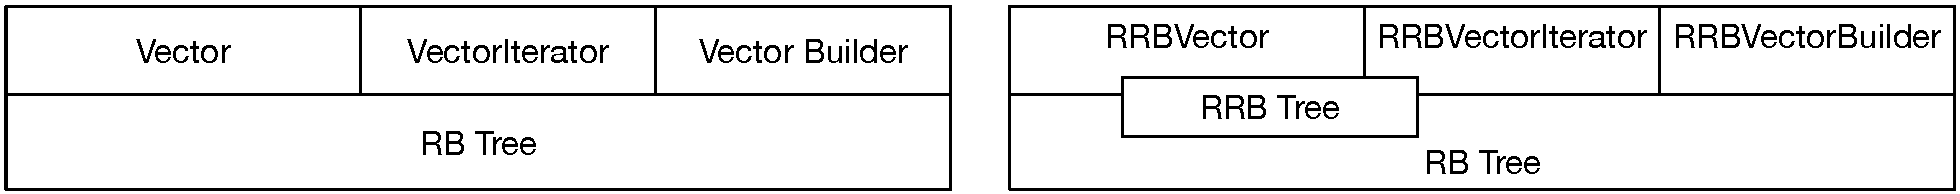
\includegraphics[width=\textwidth]{Figures/AbstractionsLayers}
  \caption{Abstractions layers for original and relaxed RB trees.}
  \label{AbstractionsLayers}
\end{figure}

%-----------------------------------
%	SUBSUBSECTION - Apply
%-----------------------------------
\subsection{Core operations with minor changes}

\paragraph{Apply}
% describe the way to get the node indices in an unbalanced node
The apply operation does not fundamentally change. The only difference is in the way the index of the next branch of a node is computed. If the node is unbalanced the sizes of the tree must be accessed (see section \ref{ComputingIndices}).


%-----------------------------------
%	SUBSUBSECTION - Updated
%-----------------------------------

\paragraph{Updated}
% doesn't change much, the sizes do not need to be updated, they jus need to be copied. Going to the correct position still may needs to access the sizes.
For the \texttt{updated} the changes are simple because the structure of the RRB-Tree will not be affected. The computation of the \texttt{indexInNode} will change to take into account the possibility of unbalanced nodes while traversing down the tree. The \texttt{copy} operation will need to copy the sizes of the node if the node is unbalanced. Because the sizes are represented in an immutable array, this copy of sizes is in fact a reference to the same object.

%-----------------------------------

\paragraph{Append}
% difference is that the the sizes may need to be updated
% performance log_32(n), remind hint of transient to amortize consecutive appends are amortised
To append an element on an RRB-Tree it is only necessary to change the \texttt{copyBranchAndAppend},  \texttt{copyAndUpdateLast} and \texttt{createNewBranch} helper functions. The \texttt{copyBranchAndAppend} will additionally copy the sizes and append to it a new size with value equal the previous last size plus one. The \texttt{copyAndUpdateLast} will also copy the sizes of the branch and increase the last size by one. The \texttt{createNew}-\texttt{Branch} will have to allocate one empty position at the end of the new non leaf nodes of the branch. Note that any new branch created by append will be created as a balanced subtree.

%-----------------------------------

\paragraph{Take}
% describe difference between the implementation (null and shift vs. cut and update size)
This operation needs to take into account the RRB tree traversal scheme to go down to the index. The tree is cut in the same way the RB-Tree is cut with an additional step. When cutting an unbalanced node the sizes of that node are cut at the same index and the last size is adjusted to match the elements in the cut. 

%-----------------------------------

\subsection{Concatenation}
% describe high level implementation in rrbvector
% performance log_32(n)
The concatenation algorithm used on RRB-Vectors is the one proposed in the RRB-Trees paper \cite{RRBTrees}. From a high level, the algorithm merges the rightmost branch of the vector on the LHS with the leftmost branch of the vector on the RHS. While merging the node, there is a rebalancing that is effectuated on each of them to ensure the logarithmic bound on the height of the vector. The RRB version of concatenation has a time complexity of $O(log_{32}(n))$, which is a clear improvement from the RB concatenation that was $O(n)$.
 \clearpage
%\lstinputlisting[]
\begin{lstlisting}[frame=single]
def concatenate(left: Vector[A], right: Vector[A]) = {
   val newTree = mergedTrees(left.root, right.root)
   val maxDepth = max(left.depth, right.depth)
   if (newTree.hasSingleBranch)
     new Vector(newTree.head, maxDepth)
   else 
     new Vector(newTree, maxDepth+1)
}
def mergedTrees(left: Node, right: Node, depth: Int) {
  if (depth==1) {
    mergedLeafs(left, right)
  } else { 
    val merged = 
      if (depth==2) mergedLeafs(left.last, right.first) 
      else mergedTrees(left.last, right.first, depth-1)
    mergeRebalance(left.init, merged, right.tail)
  }
}
def mergedLeafs(left: Node, right: Node} = {
  // create a balanced new tree of height 2 
  // with all elements in the nodes
}
\end{lstlisting}

%% describe high level algorithm
The concatenation operation starts at the bottom of the branches by merging the leafs into a balanced tree of height 2 using \texttt{mergedLeafs}. Then, for each level on top of it, the newly created merged subtree and the remaining branches on that level will be merged and rebalanced into a new subtree. This new subtree always adds a new level to the tree, even though it might be drop later on. New sizes of nodes are computed each time a node is created based on sizes of children nodes.
\begin{figure}[h!]
  \centering
  \includegraphics[width=0.8\textwidth]{Figures/Concat0.pdf}
  \caption{Concatenation example with nodes of size 4: Rebalancing level 0}
  \label{Concat0Benchmarks}
\end{figure}
%% describe branch rebalancing 
The rebalancing algorithm has two proposed variants. The first consists in completely rebalancing the nodes on the two top levels of the subtree. The second also rebalances the top two level of the subtree but it only rebalance the minimum amount of nodes that ensures the logarithmic bound. The first one leaves the tree better balanced, while the second is faster. More detail on the bounds and complexities can be bound on the RRB-Tree paper \cite{RRBTrees}. The following snippet of code shows a high level implementation of the first variant.


\clearpage
\begin{lstlisting}[frame=single]
def mergeRebalance(left: Node, center: Node, right: Node) {
  val merged = left ++ centre ++ right // join all branches
  var newRoot = new ArrayBuilder
  var newSubtree = new ArrayBuilder
  var newNode = new ArrayBuilder
  def checkSubtree() = {
    if(newSubtree.length == 32) {
       newRoot += computeSizes(newSubtree.result())
       newSubtree.clear()
     }
  }
  for (subtree <- merged; node <-subree) {
    if(newNode.length == 32) {
      checkSubtree()
      newSubtree += computeSizes(newNode.result())
      newNode.clear()
    } 
     newNode += node
  }
  checkSubtree()
  newSubtree += computeSizes(newNode.result())
  computeSizes(newRoot.result)
}

\end{lstlisting}

Figures \ref{Concat0Benchmarks}, \ref{Concat1Benchmarks}, \ref{Concat2Benchmarks} and \ref{Concat3Benchmarks} show a concrete step by step (level by level) example of the concatenation of two vectors. In the example, some of the subtrees where collapsed. This is not only to make it fit, but also to expose only the nodes that are referenced during the execution of the algorithm. Nodes with colours represent new nodes and changes, to help track them from figure to figure.


\begin{figure}[h!]
  \centering
  \includegraphics[width=0.8\textwidth]{Figures/Concat1.pdf}
  \caption{Concatenation example with nodes of size 4: Rebalancing level 1}
  \label{Concat1Benchmarks}
\end{figure}

\begin{figure}[h!]
  \centering
  \includegraphics[width=0.8\textwidth]{Figures/Concat2.pdf}
  \caption{Concatenation example with nodes of size 4: Rebalancing level 2}
  \label{Concat2Benchmarks}
\end{figure}

\begin{figure}[h!]
  \centering
  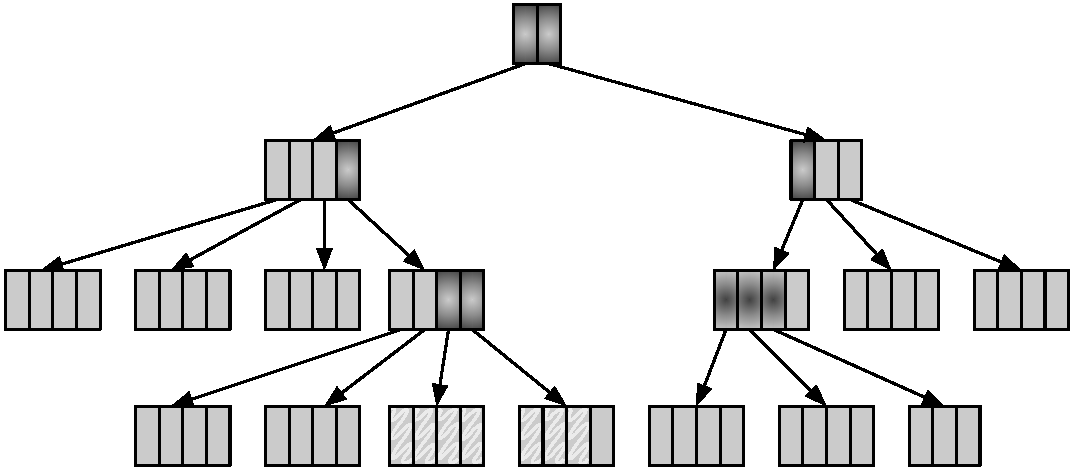
\includegraphics[width=0.8\textwidth]{Figures/Concat3.pdf}
  \caption{Concatenation example with nodes of size 4: Rebalancing level 3}
  \label{Concat3Benchmarks}
\end{figure}

% choose of algorithm
The concatenation algorithm chosen as for the RRB-Vector is the one that is slower but that rebalances better the trees. The reason behind this decision is that with better balanced trees all other operations on the trees are more performant. In fact choosing the least performant option does not need to be seen as a reduction in performance because the improvement is in relation to the RB concatenation linear complexity. An interesting consequence of the this choice, is that all vectors of size at most 1024\footnote{The maximum size of a two level RRB-Tree.} that where created by concatenation will be completely balanced.

% optimizations on small appends and prepends
When using displays and transient states, concatenating a small vector the concatenation algorithm is less performant that strait forward append or prepends on the other vector. That case is identified by using bounds on their lengths. If one is big and the other is small, a \texttt{prependAll}/\texttt{appendAll} variant is used. Those two operations are optimized version of the \texttt{append}/\texttt{prepend} that do not create the intermediate \texttt{Vector} wrapper object and some of the leaf arrays. When both vector are small enough the rebalance is done directly with \texttt{mergedLeafs}.

\paragraph{InsertAt}
% new operation
% describe simple implementation using split and concat 
% performance log_32 (from split + concat)
The operation \texttt{insertAt} is not currently defined on \texttt{Vector} because there is no way to implement it efficiently. But with RRB-Trees it is possible to implement this operation quite simply using \texttt{splitAt}, \texttt{append} and \texttt{concatenate}. This implementation has a time complexity of $log_{32}(n)$ that comes directly from the operations used.

\begin{lstlisting}[frame=single]
def insertAt(elem: A, n: Int): Vector[A] = {
  val splitted = this.splitAt(n)
  (splitted._1 :+ elem) ++ splitted._2
}
\end{lstlisting}

% hint at possible optimization by inserting directly and using transient states (take advantage of locality)
As this operation is new in the context of a vector and no real world use cases exist, this simple implementation is used\footnote{It would be possible to optimize for localized inserts on the same leaf using the same optimizations that are used for \texttt{updated}, \texttt{appended} and \texttt{prepended}}.

\subsection{Prepend and Drop}
% describe different implementation
\vskip -1em
From a high level, the \texttt{prepend} and \texttt{drop} operations on RB-Trees and RRB-Trees are quite similar. The difference is in the way the nodes are copied, updated and cut. In the RRB operations, instead of using a \texttt{startIndex}, the nodes on the leftmost branch can become unbalanced and hence represent a first branch that is not fully filled.

Most of the time, both these operation will create new unbalanced nodes, but only on the left most branch. Calling several times combinations of these two will not contribute in generating even more unbalanced branches. As such they are only responsible for the creation of at most $ log_{32}(n)$ unbalanced nodes on any vector.

\paragraph{Prepend}
Just like with the RB version, the first step is to traverse down the left most part of the tree. Traversing the tree becomes trivial because now the first branch is always on sub-index 0. As now there is a need for checking if there is still space in the leftmost branch the prepend returns a result if it could prepend it on that subtree.  

When prepending an element on a subtree, if the element was added the parent nodes are updated with there corresponding sizes. If the element could not be prepended, then we check if the root of the current subtree has still space for another branch. If there is space a new branch is prepended on it, otherwise the prepend is delegated back to the parent node.

\begin{lstlisting}[frame=single]
def +:(elem: A): Vector[A] = {
  def prepended(node: Node, depth: Int) = {
    if (depth == 1) {
      Some(copyAndPrepend(node, elem))
    } else {
      prepended(node(0), depth-1) match {
        case Some(newChild) => 
          Some(copyAndUpdate(node, 0, newChild)))
        case None if canPrependBranchOn(node) => 
          Some(copyAndPrepend(node, newBranch(depth-1)))
        case _ => None
    }
  }
  def newBranch(depth: Int): Node = {
    val newNode = Node.ofDim(2)
    newNode(0) = if (depth==1) elem else newBranch(depth-1)
    newNode
  }
  prepended(root, depth) match {
    case Some(newRoot) => new Vector(newRoot, depth, ...)  
    case None => 
      Vector(copyAndPrepend(root, newBranch(depth)), 
             depth+1, ...)
  }
}
\end{lstlisting}

Sizes are updated by adding one to each size and in the case of \texttt{copyAndPrepend} additionally prepend a 1. Nodes on new branches do not need sizes as they are balanced, but they still need the empty slot.

% Talk about balancing
This operation will generate unbalanced nodes, but will not unbalance the tree each time the \texttt{prepend} operation is called. In fact it will only generate a new unbalanced node when prepending a new branch on a balanced subtree. Then will start filling that new branch up to the point where it becomes balanced. 

% performance
% hint the displays
Due to the update of all nodes in the first branch, the complexity of this operation is $O(log_{32}(n))$. Like the RB version, \texttt{prepended} can be optimized by keeping transient states of the immutable vector \ref{sec:DisplaysTransient}).

%----------------------------------

\paragraph{Drop}
% describe difference between the implementation (null and shift vs. cut and update size)

Like with the RB-Tree \texttt{drop} operation, the first step is to traverse down the tree to the cut index. The difference is that when cutting the nodes, instead of clearing the left side of the node the node is truncated and the sizes are adjusted. For each node the adjustment is equal to the number of nodes that will be dropped in the left of the subtree. This number is already part of the computation of the cut indices on each node.  

% performance
The computational complexity of any split operation is $O(log_{32}(n))$ due to the traversal and copy of nodes on the branch where the cut index is located.

%-----------------------------------
%	SUBSUBSECTION
%-----------------------------------

\subsection{Related Structures}

\subsubsection{Vector Builder and Iterator}
\vskip -1em
The relaxation of the vector builder is discussed in section \ref{builder} and the relaxation of the vector iterator in section \ref{iterator}.

\subsubsection{Parallel Vector}
% Combine: trivial expansion from builder
%% heuristic: try to construct balanced trees 
% Split into subtrees two, take the nearest power of 32 to the half
\vskip -1em
The main difference between the RB and RRB parallel vectors is in the implementation of the combiner. This combiner is capable of combining in parallel and each combination is done in $O(log_{32}(n))$. The splitter also changed a bit to add an heuristic that helps on the performance of the combination and will tend to recreate balanced trees. 

\paragraph{Splitter}
The splitter heuristic consists in creating partitions of the tree that contain a number of elements equal to a multiple of a completely filled tree (i.e. $a \cdot 32^b$ elements). The splitter will always split into two new splitters that have a size that is as equivalent as possible taking into account the first rule. To do so, the mid point of the splitter remaining elements is identified, then shifted to the next multiple of a power of 32. This way all nodes will be full and the subsequent concatenation rebalancing will be trivial. As all nodes are full, there is no node that requires shifting elements and therefore new node creation can be avoided in some cases.

\paragraph{Combiner}
The combiner is a trivial extension of the RRB-Vector builder. It wraps an instance of the builder and for each operation of the \texttt{Combiner} that is defined in \texttt{Builder} it delegates it to the builder. The \texttt{combine} operation concatenates the results of the two builders into a new combiner. The advantages of this combiner are that the combination is done in $O(log_{32}(n))$ and that they can run in parallel on the thread pool.


I% Chapter Template

\chapter{Optimizations} % Main chapter title

\label{Optimizations} % Change X to a consecutive number; for referencing this chapter elsewhere, use \ref{ChapterX}

\lhead{\emph{Optimizations}} % Change X to a consecutive number; this is for the header on each page - perhaps a shortened title

%----------------------------------------------------------------------------------------
%	SECTION - Where does time go?
%----------------------------------------------------------------------------------------

\section{Where is time spent?}

%-----------------------------------
%	SUBSECTION 1
%-----------------------------------

\subsection{Arrays}
All nodes of the trees are represented with immutable \texttt{Array[AnyRef]}\footnote{Immutable arrays are just mutable arrays that do not get updated after initialisation.}, as this is the most compact representation for the structure and will help performance by the use of JVM primitive operations (see \ref{InPractice}). The leafs do not use specialized type arrays, as the type information is lost in methods due to generic types\footnote{Scala Collections \cite{collect11} uses generic types sequences.}, this implies that elements are already boxed when they arrive to the leafs.

% array creation, copy
Most of the memory used in the vector data structure will be composed of arrays. There are three key operations used on these arrays: array creation, array update and array access. The arrays are used as immutable arrays, as such the update operations are only allowed when the array is initialized. This also implies that each time there is a modification on some part of an array, a new array must be created and all the old elements copied.  

% size of array argument
The size of the array will affect the performance of the vector. With larger blocks (the arrays in the nodes) the access times will be reduced because the depth of the tree will decrease. But, on the other hand, increasing the size of the block will make slow down the update operations, as there is the need to copy the entire array for a single update. Benchmarks show that the sweet spot for performance is with blocks of size 32\footnote{Could also be 64, but the tradeoffs must be considered.}.


%-----------------------------------
%	SUBSECTION 2
%-----------------------------------

\subsection{Computing indices}
\label{ComputingIndices}

Computing the indices in each node while traversing or modifying the vector is key in performance. This performance is gained by using low level binary computations on the indices in the case where the tree is balanced. And, using precomputed sizes in the case where the balance is relaxed.

%-----------------------------------
\paragraph{Radix}
% Explain how to compute them
Assuming that the tree is full, elements are fetched from the tree using radix search on the index. As each node has a branching of 32, the index can be split bitwise in blocks of 5 ($2^5 = 32$) and used to know the path that must be taken from the root down to the element. The indices at each level $L$ can be computed with $(index >> (5 \cdot L)) \& 31$. For example the index 526843 would be:
\[
 526843 = 00
   	 \underbracket[0.2pt][4pt]{00000}_{\text{0}}
   	 \underbracket[0.2pt][4pt]{00000}_{\text{0}}
  	 \underbracket[0.2pt][4pt]{10000}_{\text{16}}
 	 \underbracket[0.2pt][4pt]{00010}_{\text{2}}
	 \underbracket[0.2pt][4pt]{01111}_{\text{15}}
     \underbracket[0.2pt][4pt]{11011}_{\text{27}}
\]

\begin{lstlisting}[frame=single]
def getSubIndex(indexInTree: Int, level: Int): Int = 
  (indexInTree >> (5*level)) & 31
\end{lstlisting}

% how to generalise
This scheme can be generalised to any block size $m$ where $m=2^i$ for $0 < i \leq 31$. The formula would be $(index >> (m \cdot L)) \& ((1<<m)-1)$. It is also possible to generalise for other values of $m$ using the modulo, division and power operations. In that case the formula would become $(index / (m^L)) \% m$. This last generalisation is not used because it reduces sightly the performance and it complicates other index manipulations. 

\begin{figure}[h!]
  \centering
  \includegraphics[width=0.5\textwidth]{Figures/Radix_Balanced_index_example}
  \caption{Accessing element at index 526843 in a tree of depth 5. Empty nodes represent collapses subtrees.}
  \label{radix_balanced_index_example}
\end{figure}

%-----------------------------------
\paragraph{Relaxing the Radix}
% Explain how to compute them 
When the tree is relaxed it is not possible to know the sub-indices directly from the index. That is why we keep the sizes array in the unbalanced nodes. This array keeps the accumulated sizes to make the computation of sub-indices as trivial as possible. The sub-index is the same as the first index in the sizes array where $index < sizes[subIndex]$. The simplest way to find this sub-index is by a linearly scanning the array. 

\begin{lstlisting}[frame=single]
def getSubIndex(sizes: Array[Int], indexInTree: Int): Int = {
  var is = 0
  while (sizes(is) <= indexInTree)
    is += 1
  is
}
\end{lstlisting}

% linear vs binary search
For small arrays (like blocks of size 32) this will be faster than a binary search because it takes advantage of the cache lines. If we would consider using bigger block sizes it would be better to use a hybrid between binary and linear search.

% fallback to radix
To traverse the tree down to the leaf where the index is, the sub-indices are computed from the sizes as long as the tree node is unbalanced. If the node is balanced, then the more efficient radix based method is used from there to the leaf. To avoid the need of accessing and scanning an additional array in each level.


%-----------------------------------
%	SUBSECTION 3
%-----------------------------------

\subsection{Abstractions}
\label{sec:Abstractions}
When creating an implementation for a data structure it is always a good practice to have simple abstractions to simplify the code. This makes the code easier to read an reason about but it will complicate the execution of this code. In this section we'll focus on how the actual implementation optimises out overheads that would be generated by functions and generic code abstractions.

% functions
\paragraph{Functions} When writing an algorithm we usually divide it into small self-contained subroutines and we try to factor out the common ones. In practice this will add overhead for function invocations each time a function is used and break the locality of the code. To improve the performance we avoid as much as possible function call on simple operations. The code also avoids the creation of any higher order function to avoid additional object allocations. As such \texttt{while} loops are used rather than \texttt{for} loops.

%-----------------------------

\paragraph{Generalization}
A common way to reduce the amount of code that needs to be written when implementing common functionality is using generalization of code. But this comes with a computational cost for cases where a second implementation that takes into account the context of to simplify the operation. When considered beneficial the code is specialized by hand on the current context\footnote{This is specialisation on value.}. 

% generic code vs specialized code (specialized values, expanded loops)
The base mechanisms to specialize are: specialisation of a value, loops unrolling and arithmetic simplifications. Value specialization consist in explicitly identifying the value of some field and then using code specialized on that value. Loop unrolling (including recursions) consist in writing explicitly the code for each loop instead of the loop. This one is usually used on loops that are bounded by some value specialization. Once the first two specialisation are applied code can be simplified with arithmetic transformations. 

% example with simple expanded get operation (show expansion and specialisation)
Concretely, most of the value specialization is done on heights and indices on radix operations. The height are a bounded small range of numbers and therefore can be efficiently specialized with a \texttt{match}\footnote{All \texttt{match} expressions used in this specialization get compiled to \texttt{tableswitch} bytecode instruction. In some cases it would be beneficial to have  \texttt{tableswitch} with fallthrough, but the there is currently no Scala construct that compiles to that.} expression. On ranges of indices that are on trees of the same size specialization is done using nested \texttt{if/else} expressions. It is also possible to specialize of the first and last index, the first index (the 0 index) gains much from specialization because of arithmetic cancelation of terms. As an example here is a version of the radix \texttt{apply}. 

\begin{lstlisting}[frame=single]
def apply(index: Int): A = {
    vectorDepth match {
      case 1 => 
        vectorRoot(indexInNode & 31)
      case 2 => 
        val node1 = vectorRoot((indexInNode>>5) & 31)
        node1(indexInNode & 31)
      case 3 => 
        val node2 = vectorRoot((indexInNode>>10) & 31)
        val node1 = node2((indexInNode>>5) & 31)
        node1(indexInNode & 31)
      case 4 =>
        ...
    }
  }
\end{lstlisting}

Where the \texttt{vectorDepth} is specialized, then the recursion is rolled and finally a \texttt{>>} is removed on each branch of the \texttt{match}. Taking this one setup further with the \texttt{head} method that is usually implemented as \texttt{apply(0)}, using the same specialization, removing the need for any additional arithmetic operation, the code becomes:

\begin{lstlisting}[frame=single]
def head(): A = {
    vectorDepth match {
      case 1 => vectorRoot(0)
      case 2 => vectorRoot(0)(0)
      case 3 => vectorRoot(0)(0)(0)
      ...
    }
  }
\end{lstlisting}

In relaxed radix operation the loop unrolling is usually avoided because in those methods the amount of nodes traversed can't be known in advance. But will invoke specialized versions of the code as soon as it finds a node on which it is possible. For a perfectly balanced RRB-Tree that node is to root, and hence the performance for such vectors is similar to the one for an RB-Tree.

%----------------------------------------------------------------------------------------
%	SECTION - Displays
%----------------------------------------------------------------------------------------
\clearpage
\section{Displays}
\label{sec:Displays}
% describe display fields in vector object
As base for optimizations, the vector object keeps a set of fields to track one branch of the tree. They are named with using the level number from 0 up to the maximum possible level. In the case of blocks of size 32 the maximum level used is 5\footnote{As in practice, only the 30 bits of the index are used.}, they are allocated by default and nulled if the tree is shallower. The highest non null display is and replaces the root field. All displays bellow the root are never null. This implies that the vector will always be focused on some branch.

\begin{figure}[h!]
  \centering
  \includegraphics[width=0.8\textwidth]{Figures/Displays}
  \label{Displays}
  \caption{Displays}
\end{figure}

% describe the focus field
To know on which branch the vector is focused there is also a \texttt{focus} field with an index. This index is the index of any element in the current \texttt{display0}. This index represents the radix indexing scheme of node sub-indices described in \ref{ComputingIndices}. 

% immutability of displays
To follow the simple implementations scheme of immutable objects in concurrent contexts, the focus is also immutable. Therefore each vector object will have a single focused branch during its existence\footnote{The display focus may change during the initialisation of the object as optimisation of some methods}. Each method that creates a new vector must decide which focus to set. 

%-----------------------------------
%	SUBSECTION As cache
%-----------------------------------

\subsection{As cache}
% used to access some elements directly from the smaller subtrees (XOR)
One of the uses of the displays is as a cached branch. If the same leaf node is used in the following operation, there is no need for vertical tree traversal which is key to amortize operation to constant time. In the case another branch in needed, then it can be fetched from the lowest common node of the two branches. 

% xor
To know which is the level of the lowest common node in a vector of block size $2^m$ (for some consistent $m$), only the \texttt{focus} index and the index being fetched are needed. The operation \texttt{index\^{ }focus} will return a number is bounded to the maximum number of elements in a tree of that level. The actual level can be extracted with some if statements. This operation bounded by the same number of operations that will be needed to traverse the tree back down through the new branch.

\begin{lstlisting}[frame=single]
def getLowestCommonLevel(index: Int, focus: Int): Int = {
  val xor = index ^ focus
  if (xor < 32 /*(1<<5)*/ ) 0
  else if (xor < 1024 /*(1<<10)*/ ) 1
  else if (xor < 32768 /*(1<<15)*/ ) 2
  ...
  else 5
}
\end{lstlisting}

% keeping relevant branch for next operations
When deciding which will be the focused branch of a new vector two heuristics are used for this: If there was an update operation on some branch where that operations could be used again, that branch is used as focus. If the first one cant be applied, the display is set to the first element as this helps key collection operations such as \texttt{iterator}.

%-----------------------------------
%	SUBSECTION  For transient states
%-----------------------------------

\subsection{For transient states}
\label{sec:DisplaysTransient}
% operation: append, prepend, update
Transient states is the key optimisation to get append, prepend and update to amortized constant time. It consists in decoupling the tree by creating an equivalent tree that does not contain the edges on the current focused branch. The information missing in the edges of the tree is represented and can be reconstructed from the displays. In the current version of the collections vector \cite{scalaVector211} this state is identified by the \texttt{dirty} flag\footnote{In the RRB Vector \cite{projecRepo} implementation it was replaced by \texttt{transient}.}.

\begin{figure}[h!]
  \centering
  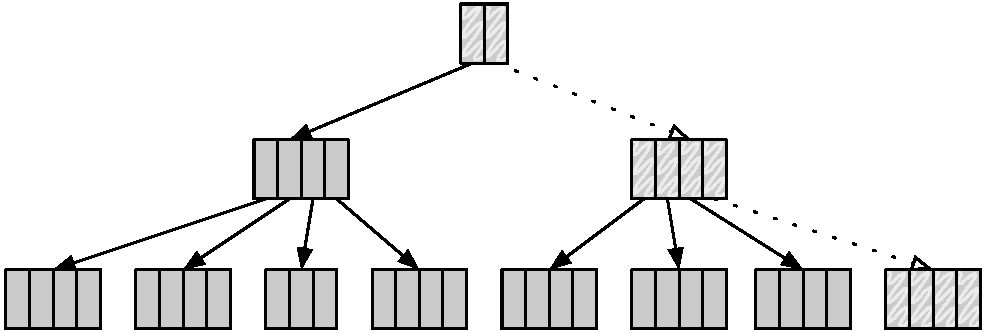
\includegraphics[width=0.8\textwidth]{Figures/Transient_state}
  \label{Transient_state}
  \caption{Transient Tree with current focus displays marked in white and striped nulled edges.}
\end{figure}

% transient states are used to amortized operations
Without transient states when some update is done on a leaf, all the branch must be updated. On the other hand, if the state is transient, it is possible to update only the subtree affected by the change. In the case of updates on the same leaf, only the leaf must be updated. When appending or prepending, $\frac{31}{32}$ operations must only update the leaf, then $\frac{31}{1024}$ need to update two levels of the tree and so on. These operations will thus be amortized to constant ($\sum_{k=1}^{\infty} \frac{k*31}{32^k} = \frac{32}{31}$ block updates per operation) time if they are executed in succession.

% normailization
There is a cost associated to the transformation from canonical to transient state and back. This cost is equivalent to one update of the focused branch. The transient state operations only start gaining performance on the canonical ones after 3 consecutive operations. With 2 consecutive operations they are matched and with 1 there is a loss of performance.

%-----------------------------------
%	SUBSECTION  Relaxing the Displays
%-----------------------------------

\subsection{Relaxing the Displays}
% describe fundamental difference in the focus (focused on balanced subtree)
When relaxing the tree balance it is also necessary to relax the displays. This is mainly due to the loss of a simple way to compute the lowest common node on unbalanced trees. Computing the node requires now the additional sizes information located in each unbalanced node. As such it is necessary to access the nodes to be able to compute the lowest common node, and there is a loss in performance due to increased memory accesses.  

% describe focus start, focus end and focus (focus relaxed)
To still take advantage of efficient operations on balanced trees, the display is relaxed to be focused on a branch of some balanced subtree\footnote{A fully balanced tree will be itself the balanced subtree, as such it will always use the more performant operations.}. To keep track of this subtree there are three additional fields: \texttt{focusStart} that represents start index of the current focused subtree, \texttt{focusEnd} that represents the end index of the subtree and \texttt{focusDepth} that sets  height of the focused subtree\footnote{As an optimisation, the \texttt{focus} field is split into the part corresponding to the subtree and the part that represents the indices of the displays that are unbalanced.}. The operations that can take advantage of the the efficient display operations will check if the index is in the subtree index range and invoke the efficient operation. If not, it will invoke the relaxed version of the operation, that starts from the root of the tree.

% describe how fetching elements change
For example, the code for \texttt{apply} would become:
\begin{lstlisting}[frame=single]
def apply(index: Int): A = {
  if (focusStart <= index && index < focusEnd) 
    getElementFromDisplay(index - focusStart)
  else if (0 <= index && index < endIndex) 
    getElementFromRoot(index)    
  else 
    throw new IndexOutOfBoundsException(index)
}
\end{lstlisting}

This \texttt{apply} method on the unbalanced subtrees of figure \ref{Balanced_subtrees}  would use the \texttt{getElementFromDisplay} to fetch elements in \texttt{display0} directly from it and fetch elements from nodes (1.1) and (1.2) starting from \texttt{display1}. The rest is fetched from the root using \texttt{getElementFromRoot}.

\begin{figure}[h!]
  \centering
  \includegraphics[width=\textwidth]{Figures/Balanced_subtrees}
  \caption{Relaxed Radix Balanced Tree with a focus on a balanced subtree rooted of \texttt{display1}. Light grey boxes represent unbalanced nodes sizes.}
  \label{Balanced_subtrees}
\end{figure}

%-----------------------------------
%	SUBSECTION  Vector Canonicalization
%-----------------------------------

\subsection{Vector Canonicalization}
\label{VectorCanonicalization}
% State can mutate from transient to canonical exactly once (similar to lazy evaluation)
% State mutation is not visible from outside
% If more performance is requires it is possible to write transient state operations directly to transient state

\begin{figure}[h!]
  \centering
  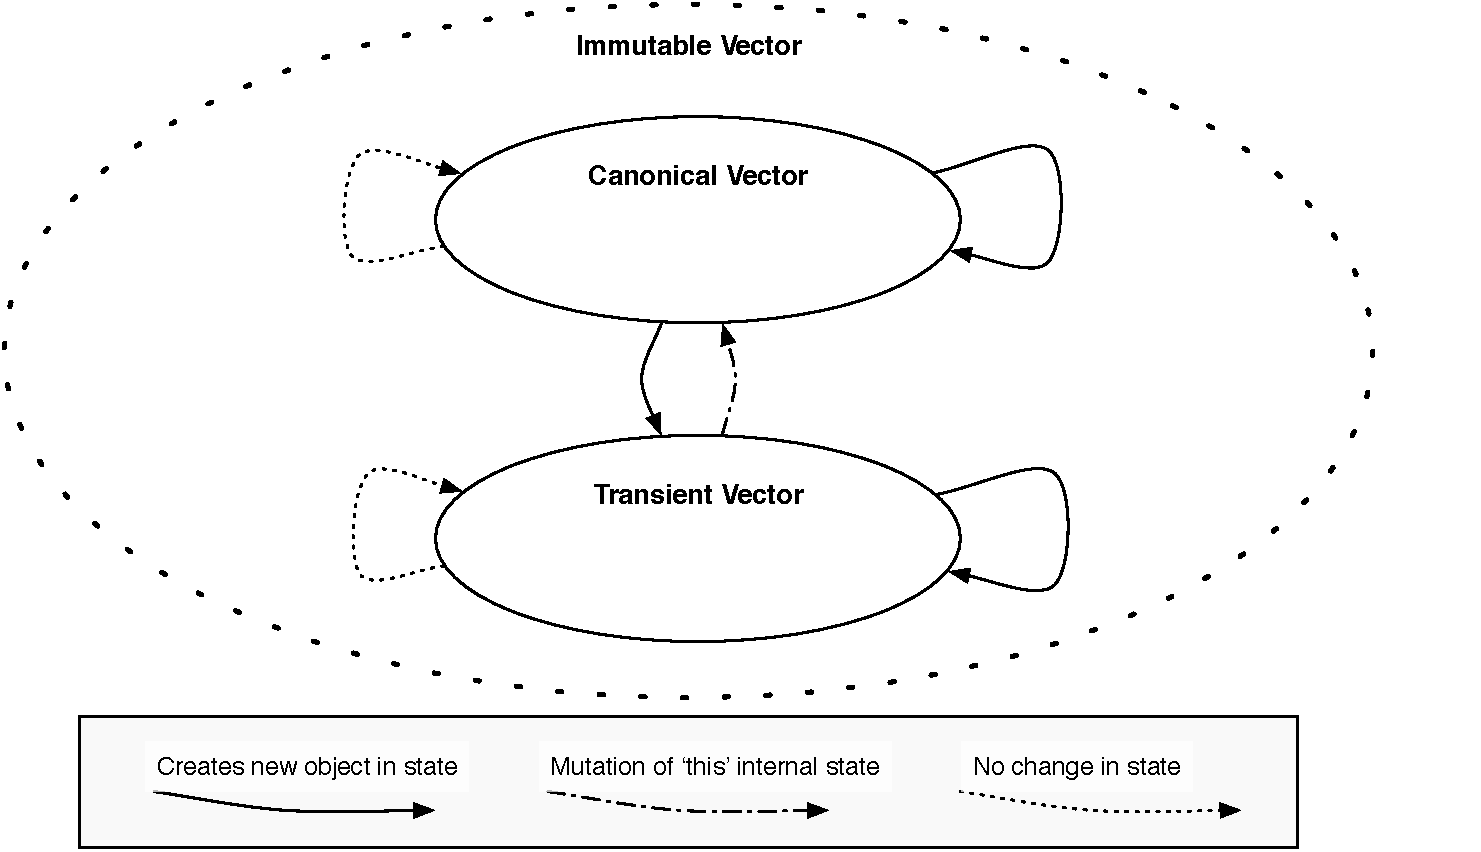
\includegraphics[width=0.8\textwidth]{Figures/StatesGraphRealySimple}
  \caption{Objects states and effect of operations.}
  \label{StatesGraphRealySimple}
\end{figure}

As stated in section \ref{sec:DisplaysTransient} vectors have two representations: canonical and transient. The transient state aims to improve performance of some operations by amortising costs. But, the transient state is not ideal for performance of other operations. For example an \texttt{apply} operation on an unbalanced vector may lack the sizes information it requires to access certain indices. And an iterator relies on a canonical tree for performance. It is always possible to implement those operations on transient states, but they would involve additional overhead on each call and duplication of code.

The solution is to convert the transient representation to a canonical one when an operation that requires it is called on an instance of the immutable vector. The mutation of the vector is not visible from the outside and only happens at most once (see figure \ref{StatesGraphRealySimple}). This transformation only affects the nodes that are on the display, it copies each one (except the leaf) and links the trees. If the node is unbalanced, the size of the subtree in focus is inserted. This transformation could be seen as a lazy initialization of the current branch.

\begin{figure}[h!]
  \centering
  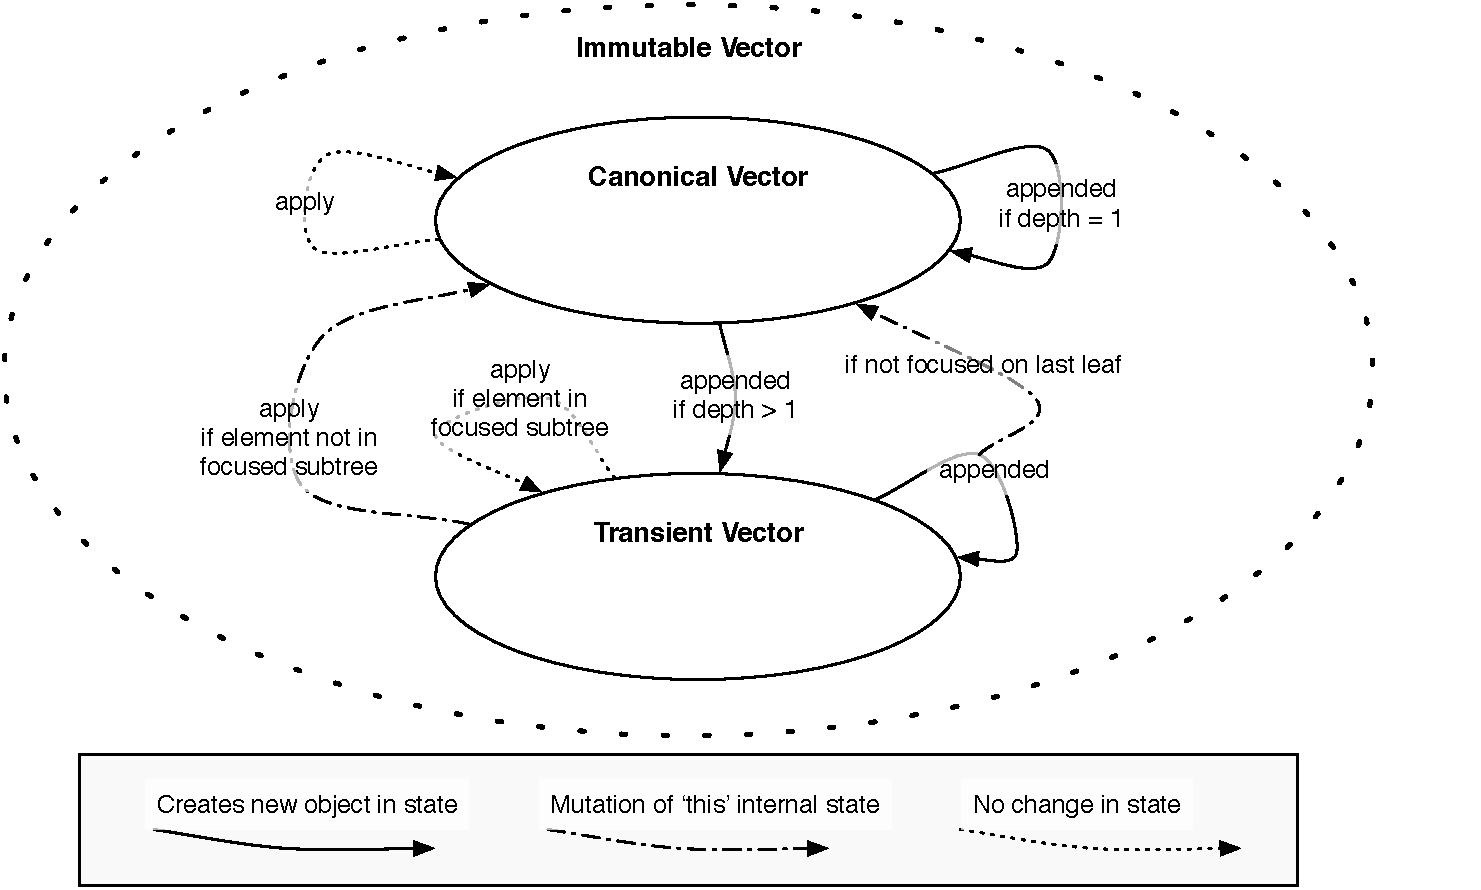
\includegraphics[width=0.8\textwidth]{Figures/StatesGraphSimple}
  \caption{Transient state creation and canonicalization of vectors for \texttt{append} and \texttt{apply} operations.}
  \label{StatesGraphSimple}
\end{figure}

% Explain append/prepend
Vector objects can only be in transient state if they where created that way. For example, the \texttt{append}/\texttt{prepend} operation will create a new object that is in transient state and focused on the last/first branch. If the source object was not focusing the last branch, then it is canonicalized (if needed) before change of branch operation. Vectors depth 1 are special cases, they are always in canonical form and their operations are equivalent to those in transient form.

Figure \ref{StatesGraphSimple} shows the different states and the effects of the \texttt{append} and \texttt{apply} operations on them. Figure \ref{StatesGraphComplete} shows the same for all operations. Note that the mutation of \texttt{this} object only happened from transient to canonical and that the only way to get to transient is with the creation of a new vector object.

\begin{figure}[h!]
  \centering
  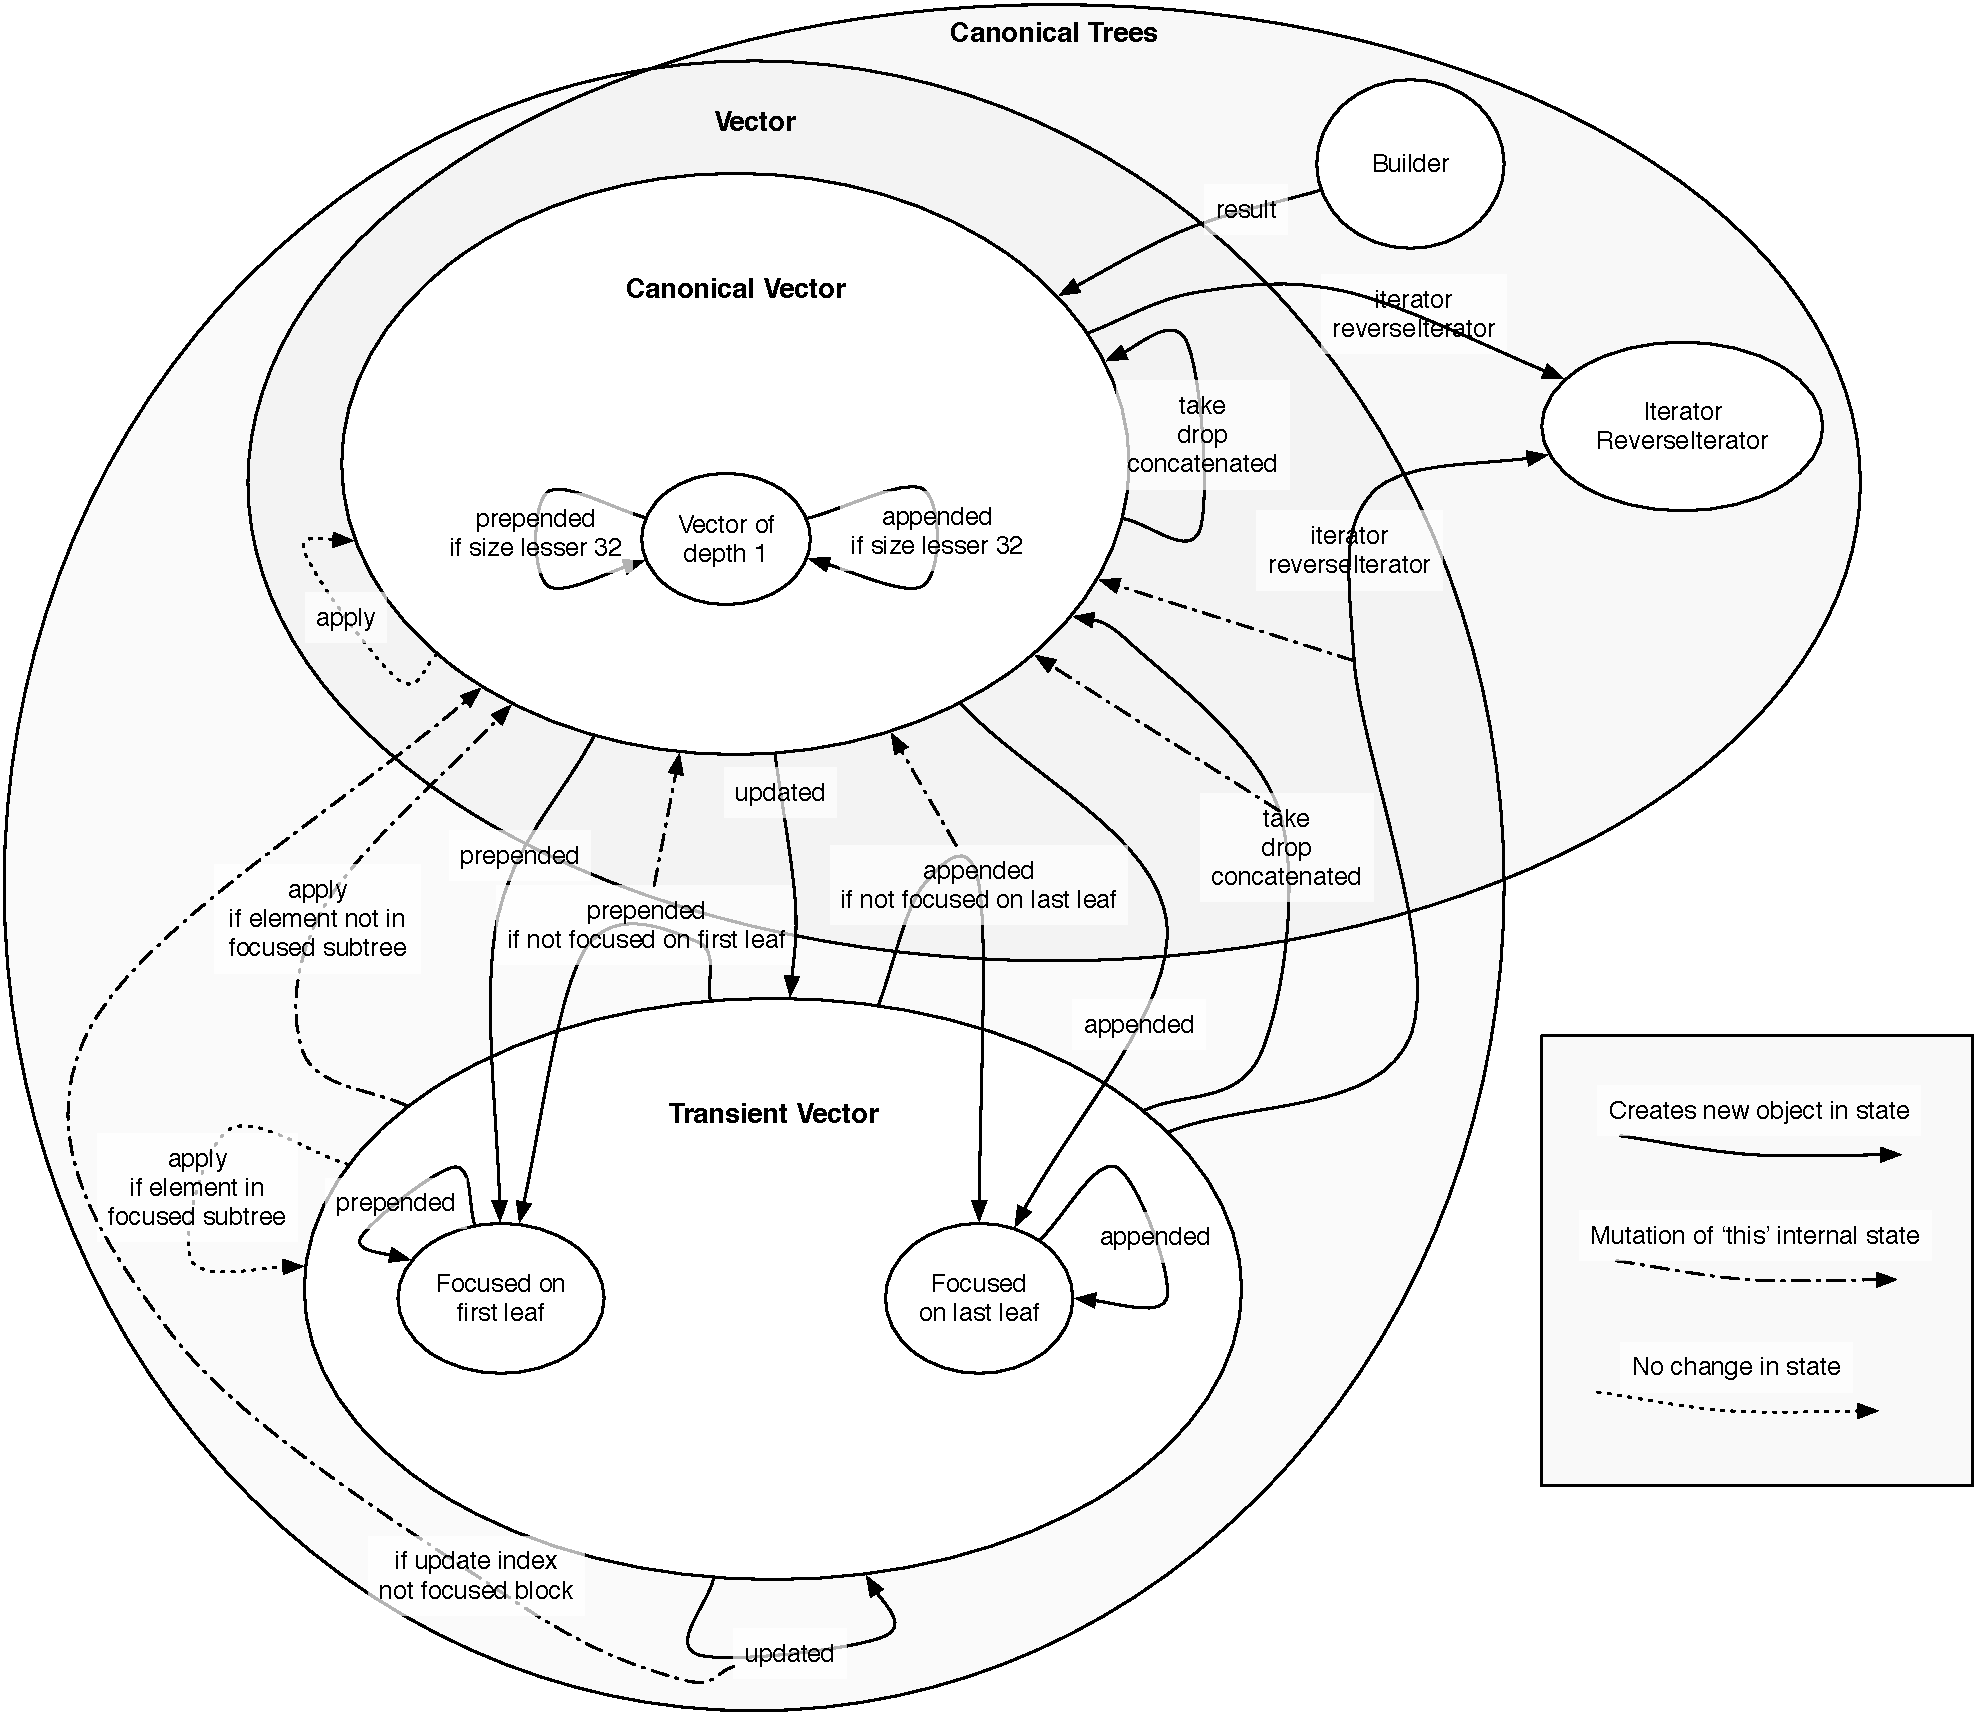
\includegraphics[width=\textwidth]{Figures/StatesGraph}
  \caption{Transient state creation and canonicalization of vectors for every operation.}
  \label{StatesGraphComplete}
\end{figure}

%----------------------------------------------------------------------------------------
%	SECTION - Builder
%----------------------------------------------------------------------------------------
\clearpage
\section{Builder}
\label{builder}
% use of mutable tree 
% avoid creation unnecessary arrays
A vector builder is a special wrapper for a RB-Tree that has an efficient \texttt{append} operation. It is implemented using encapsulated mutable arrays during the building of the vector and then frozen on the creation of the result. Any array that the builder can still mutate is cloned and possibly truncated to generate the RB-tree of the vector. 

The benefits of the mutable \texttt{append} operation of the builder over \texttt{appended} operation of the vector are on the reduced amount of memory allocations needed in the process of appending. There is no need to allocate a new \texttt{Vector} object each time an element is appended. Even more important is that there is no need to create a new array in each change on a node, nodes are allocated once and filled as needed. 

%-----------------------------------
\paragraph{Relaxing the Builder}
% same base implementation for +=
% addition of accumulator for  ++= 
Most of the operations implemented in the collections framework that use builder usually create the new collection by appending one element at a time. To retain the performance of all existing operation that use builders the implementation builder append does not change. Therefore the tree where elements are appended is always perfectly balanced.
 
 To add performance when concatenating a \texttt{Vector} to a builder a new field is added to retain a vector that will be lazily concatenated to the result. This vector is the accumulation \texttt{acc} of all elements (or all vectors) that where added before (and including) the last concatenation and elements in the current tree been build. All elements added after the last concatenation are added to the main the mutable tree of the builder.


%----------------------------------------------------------------------------------------
%	SECTION - Iterator
%----------------------------------------------------------------------------------------
\clearpage
\section{Iterator}
\label{iterator}
% efficient tree traversal vs iteration by index
% avoid re-traversing vertically the tree from the root
The default implementation for iterator in \texttt{IndexedSeq} is by iterating on the indices and accessing elements with the \texttt{apply} method. This is not optimal because it requires traversing the tree down from the root each time an element is accessed. The traversal of the vector using this would have a computational complexity of $O(n \cdot log_{32}(n))$.

To improve performance of the iteration on vector a normal tree traversal of the underlying RB-Tree amortizes the computational complexity to $O(n)$. The iterator can use the display optimization to keep track of the current branch and move to the next branches efficiently using the radix index scheme. In this case the display is allowed to mutate. The current implementation of vector is implemented this way\footnote{The current \texttt{reverseIterator} is still using traversal by index.}. 

%-----------------------------------
\paragraph{Relaxing the Iterator}
% same implementation within a balanced subtree
% refocus from root to iterate between balanced subtrees
To keep the performance advantages of the tree traversal on balanced RRB-trees, iteration is done the same on every balanced subtree. When the end of a balanced subtree is reached the first element of the next balanced subtree is focused and the traversal continues efficiently from there. If the tree is not too unbalanced the traversal will tend to be $O(n)$. But if the tree is extremely unbalanced it will tend to fall back on $O(n \cdot log_{32}(n))$, where the additional $log_{32}(n)$ comes from the changes of balanced subtrees. Even in this bad last case the performance is better than the traversal by index because each leaf is a balanced subtree, on which efficient traversal is used. The RRB-Vector implements both \texttt{iterator} and \texttt{reverseIterator} this way.






 
I% Chapter Template

\chapter{ Performance in Practice} % Main chapter title

\label{Performance} % Change X to a consecutive number; for referencing this chapter elsewhere, use \ref{ChapterX}

\lhead{\emph{Performance in Practice}} % Change X to a consecutive number; this is for the header on each page - perhaps a shortened title


%----------------------------------------------------------------------------------------
%	SECTION In practice: Running on JVM
%----------------------------------------------------------------------------------------
\section{In practice: Running on JVM}
\label{InPractice}

In practice, Scala compiles to Java bytecode and executes on a JVM, where we take the Java SE HotSpot as a reference. This imposes additional characteristics of performance that can't be evaluated on the algorithmic level alone.

% code interpreted vs compiled
The JVM use \emph{just in time} (or JIT) compilation of code to take advantage of knowledge about how the code is used at runtime. At first it runs on interpreter mode, it consists of interpreting the bytecode and collecting statistics on the codes execution. Eventually it will compile the code to make it faster using several optimizations and heuristics. The code of the vectors tries to gains performance by aligning with those heuristics and hence taking advantage of the JVM optimizations.

% GC and memory allocations
One of the components of the JVM that will be affected by vectors is the garbage collector. The vector tends to create a large amount of \texttt{Arrays} during transformations, of which many are only necessary for a short time. Those objects will use up memory and possibly degrade performance of future allocations, until the next GC. Having all these unused object will also contribute in an increase in the frequency of GC executions. For that reason the code is optimized to avoid excessive creation of intermediary objects.

% memory access and caches
% system arraycopy primitive
When running on some machine we have several memory cashes helping with performance. The vector tries to align to the underlying cache model to improve performance. The size of the arrays is chosen to take advantage of cache lines while they are copied and traversed. This makes the behaviour of node copies look more as a constant time operation. Further more when copying arrays the \texttt{System.arraycopy} primitive is used. This way, the critical operation that is executed on each update will use the lowest level implementation available for the JVM. This could potentially go down to efficient host machines code when compiled.

%-----------------------------------
%	SUBSECTION Cost of Abstraction
%-----------------------------------
\subsection{Cost of Abstraction and JIT Inline}
% cost of function invokation
One of the optimizations that the JVM provides is function call elimination (abstraction elimination) based on a set of heuristics. This is equivalent to the functions optimization in section \ref{sec:Abstractions} but done on another level of the pipeline. Critical parts of the code are written with careful detail to match the heuristics of the JVM. 

% code compiled (inlined if hot)
% aim to make all critical methods 35< bytes
The optimisation works as follows: the code is run in interpretation mode first while keeping track of statistics on which parts of the code are executed and how many times. When the code is eventually compiled, function calls that are deemed \emph{hot} are inlined. The heuristic favours inline when the function has less than 35 bytes. 

We use this knowledge of the heuristic in two ways. The first is to avoid inlining everything, if the function is small and there is no other optimization that can be done if inline manual, the code is kept as a function. The second is to inline the methods of the vector API into the clients code. When implementing functions with less than 35 bytes, performance was tested and cross referenced with the VMs inlining diagnostic\footnote{The JVMs \texttt{"-XX:+UnlockDiagnosticVMOptions -XX:+PrintInlining"} flag was used to track the inlining.}. The code was inspected using \texttt{javap -c}, which gives the sizes of the function and helped identifying some optimization possibilities.

%----------------------------------------------------------------------------------------
%	SECTION Scalameter
%----------------------------------------------------------------------------------------
\clearpage
\section{Measuring performance}
% Scalameter
ScalaMeter framework\cite{scalameter} is used to measure performance of operations on different implementations of vector. This framework was used to spot identify performance improvements or regressions during the development process. 

% warmup to compile code and reduce jitter (JIT, GC)
To have reproducible results with low error margins, ScalaMeter was configured on a per benchmark basis\footnote{The JVM \texttt{-XX:+PrintCompilation} flag vas used to help identifying the ideal configuration.}. Each test is run on 32 different JVM instances to average out badly allocated VMs. On each JVM 32 measurements are taken, while using outlier elimination to remove benchmark runs that where exceptionally different. This could happen if one particular run has a garbage collection, JIT compilation of code or OS executing something else. Before the benchmark runs the JVM is warmed up by running some times the benchmark without taking measurements. During these first execution the VM will be loading classes, taking some statistic on the code and then eventually compiling it.

% types of vectors
There are two main axis of performance comparisons. The first is between the RB-Vector and a perfectly balanced RRB-Tree where the aim is to have an equivalent performance, even if the RRB-Vector have an inherent additional overhead. The second axis is the one that shows the effects of unbalanced nodes on RRB-Tree. For this we compare the same perfect balanced vector with one that is the result of one concatenation of two vectors and with an extremely unbalanced vector. The later vector is generated by concatenating random\footnote{Pseudo random generator where used to be able to reproduce the same ones each time.} small vectors together. The amount of unbalanced nodes is in part affected by the size of the vector. Other axes are discussed in the next section.

%----------------------------------------------------------------------------------------
%	SECTION Generators
%----------------------------------------------------------------------------------------
\clearpage
\section{Implementation Generators}
\label{ImplementationGenerators}
Until now only one implementation of the RRB-Vector\footnote{Located in the \texttt{scala.collection.immutable.rrbvector} package on GitHub} that is compared against the RB-Vector. But in fact to compare performance on different characteristics like block sizes and concatenation algorithm variant concrete implementations where generated using Scala reflection. Other characteristics involve a complete structure assertion while testing and benchmarks generation. For each combination of characteristics there is a concrete artefact: class implementation, tests and benchmarks.

Code is generated by combining AST using Quasiquotes with some domain specific optimizations. The optimizations are the same that where applied manually on the main implementation of the RRB-Vector. The resulting code is equivalent, except that it lacks formatting. The name of the artefact is used to identify the different characteristics\footnote{All generated artefacts are in the \texttt{scala.collection.immutable.generated.rrbvector} package on GitHub}.

% block sizes
The block sizes used where 32, 64, 128 and 256. 
The main aim is the differences in performances of the operations and identify sizes for which permanence degrades due to loss of cache locality. 
This is the only number in the name of the artefact.

% concat implementation
Both version of the RRB-Vector are to generate vectors. 
This done mostly to compare the performances of other operation on vector that got unbalanced using concatenation. 
\texttt{Complete} (or \texttt{c} in the name of the artefact) is used to name identify the version that rebalances completely the subtree. 
The other one is named \texttt{Quick} or \texttt{q} in the name of the artefact.

% testing
For testing purposes, for each implementation there is a second one generated with heavy assertions on the whole structure of the vector on most methods (see \ref{InvariantAssertions}). 
Concrete benchmarks are also generated at the same time.

Generating this code was the only reasonable way to implement this huge amount of classes while implementing new features on them. 
Changes that would otherwise had to be propagated by hand on each one. 
This also help to find and fix bugs, because a bug has a higher probability of affecting at leas one of the artefact and a fixed bug fixes it on all of them.

%----------------------------------------------------------------------------------------
%	SECTION Benchmarks
%----------------------------------------------------------------------------------------
\clearpage
\section{Benchmarks}
% reiterate the the different benchmark types 
%% differences between implementation (vector vs rrbvector)
%% differences between unbalances
%% differences between block sizes
%% differences between concatenation rebalancing method
% benchmarks on core operations
Performance benchmarks aim to compare the performance of all core operations of the vectors RRB-Trees. These operations are: \texttt{apply}, \texttt{concatenate}, \texttt{append}, \texttt{prepend}, \texttt{take}, \texttt{drop}. The performance of specialized operations for the iterators, builder and the parallel vector where also benchmarked. Additionally, the memory footprint of different vectors was checked.

The axis of comparisons are: 
\begin{itemize}
	\item Size of the vector. Split into ranges that correspond to vectors of the same height, when perfectly balanced.
	\item \texttt{Vector} against completely balanced \texttt{RRBVector}
	\item Differently balanced \texttt{RRBVector}s: perfectly balanced, unbalanced (by one concatenation) and extremely unbalanced. This is ignored on vector of depth lesser than 3 because there all those vectors end up being perfectly balanced.
	\item Different block sizes: 32 (original), 64, 128 and 256.
	\item Different implementation of the rebalancing in \texttt{concatenate}: Complete rebalance and Quick rebalance
	\item Thread pool size for parallel vectors.
\end{itemize}

% machine description
For the results of this sections, All benchmarks where executed on a Java HotSpot(TM) 64-Bit Server VM on a machine with an Intel(R) Core(TM) i7-4770 CPU @ 3.40GHz with 32GiB on RAM. Each benchmarking VM instance was setup with 16GiB of heap memory. 

%-----------------------------------
%	SUBSECTION Apply
%-----------------------------------
\subsection{Apply}
% describe the benchmark function
The \texttt{apply} benchmarks aim to see the amortized access time of elements. Amortizing the displays optimization and memory caches. For this, each benchmark invokes the \texttt{apply} operation $10k$ times on different elements. 

There are two variants: the first variant access the elements sequentially and the second one chooses each time a random index. The first one is supposed to have better performance because the array that are access tend to be in cache. The computations of the next index is also a bit more complex on the second one, but mostly irrelevant compared with the cache misses of all the arrays on a branch.

% compare expectation with results
% explain the upper bound
The benchmark results for the sequential access in figures \ref{ApplyBenchmarks2} and \ref{ApplyBenchmarks3} show that if the RRB-Vector is balanced or just slightly unbalanced will be faster than the RB-Vector. But when it gets extremely unbalanced the performance can drop by around 0.5X which is proportional to the increase of arrays that must be accessed (two per node).

\begin{figure}[h!]
  \centering
  \includegraphics[width=\textwidth]{Benchmarks/Apply_2.pdf}
  \caption{Time to execute 10k apply operations on sequential indices on vectors of height 2.}
   \label{ApplyBenchmarks2}
\end{figure}

The performance improvements where achieved by analysing the sizes of the functions involved, there inlining and which parts of the code is used in each case. The aim was to improve performance of unbalanced vectors, that is why in some cases the slightly unbalanced vector is the faster. 

\begin{figure}[h!]
  \centering
  \includegraphics[width=\textwidth]{Benchmarks/Apply_3.pdf}
  \caption{Time to execute 10k apply operations on sequential indices on vectors of height 3.}
   \label{ApplyBenchmarks3}
\end{figure}

\FloatBarrier

Figure \ref{ApplyRandomBenchmarks} show the results for random indices. It can be observed that the behaviour of the curve is quite similar, but the sequential one is around 2X faster due to memory locality.

\begin{figure}[h!]
  \centering
  \includegraphics[width=\textwidth]{Benchmarks/Apply_random_3.pdf}
  \caption{Time to execute 10k apply operations on random indices on vectors of height 3.}
  \label{ApplyRandomBenchmarks}
\end{figure}

\FloatBarrier

Finally, the figures \ref{ApplyBlocksBenchmarks} show what would happen if the block sizes changed or if the rebalance algorithm is changed. Note that in the cases for blocks of 128 and 256 the complete rebalance is actually creating completely balanced vectors. It can be observed that the quick rebalance is harmful to the performance of the apply method. Increasing the sizes of the arrays will improve the performance of the apply method.

\begin{figure}[h!]
  \centering
  \includegraphics[width=0.49\textwidth]{Benchmarks/Apply_blocks_32.pdf}
  \includegraphics[width=0.49\textwidth]{Benchmarks/Apply_blocks_64.pdf}
  \includegraphics[width=0.49\textwidth]{Benchmarks/Apply_blocks_128.pdf}
  \includegraphics[width=0.49\textwidth]{Benchmarks/Apply_blocks_256.pdf}
   \caption{Time to execute 10k apply operations on sequential indices. Comparing performances for different block sizes and different implementation of the concatenation inner branch rebalancing (Complete/Quick).}
  \label{ApplyBlocksBenchmarks}
\end{figure}

\FloatBarrier

%-----------------------------------
%	SUBSECTION Concatenation
%-----------------------------------
\subsection{Concatenation}
% describe the benchmark function
The \texttt{concatenation} benchmarks aim to show the benefit of having the logarithmic concatenation algorithm against the linear version. The benchmarks concatenate two vectors of the same type and balance characteristics. As such these benchmarks have two axis representing the sizes of the LHS and RHS vector in the operation.


% compare expectation with results
% explain the upper bound
% explain apparently incoherent results

Figure \ref{ConcatBenchmarks} shows how the concatenation time for RB-Vectors is linear on the size of the resulting vector. Below that, the three surfaces that represent the RRB-Vector concatenation are effectively constant time (or $log_{32}(n)$). The performance difference between the differently balanced RRB-Vectors is negligible in relation to the difference with RB-Vector. 

\begin{figure}[h!]
  \centering
  \includegraphics[width=\textwidth]{Benchmarks/Concat.png}
  \caption{Execution time for a concatenation operation on two vectors. In theory (and in practice) Vector concatenation is $O(left + right)$ and the rrbVector concatenation operation is $O(log_{32}(left + right))$.}
   \label{ConcatBenchmarks}
\end{figure}

In the case of concatenation, being balanced or not does not impose performance improvements or degradations. Performance will be determined by the number elements in the branches that get merged and their alignment.

The benchmark for the Quick rebalancing version where not included here because the implementation for that one is suboptimal and the comparison would not be fair. The main purpose of that version is to show the differences it would cause on other operation. The current version of the Quick rebalancing can achieve 2X performance benefit, but it could gain a lot form the same optimizations that were used on the Complete rebalancing.

\FloatBarrier

%-----------------------------------
%	SUBSECTION Append
%-----------------------------------
\subsection{Append}
% describe the benchmark function
The \texttt{append} benchmarks aim to see the amortised time taken to appending elements. With the transient states, the branch updates are amortized over leaf updates. For this, each benchmark appends 256 elements on a vector. This way there is at least one branch update for each benchmark, 8 if the block size is 32.

\begin{figure}[h!]
  \centering
  \includegraphics[width=\textwidth]{Benchmarks/Append_2.pdf}
  \caption{Time to execute 256 append operations on vectors of height 2. This shows the amortized cost of the append operation.}
  \label{Append2Benchmarks}
\end{figure}

% compare expectation with results
% explain the upper bound
% explain apparently incoherent results
The figures \ref{Append2Benchmarks} and \ref{Append3Benchmarks} show that if the RRB-Vectors are balanced or just slightly unbalanced the execution time is equivalent to the one for RB-Vectors. But, if it gets extremely unbalanced the performance can fall to by 0.6X. In figure \ref{Append2Benchmarks} it is possible to see that after 768 the performance does a step upward, this correspond to the addition of a level in the tree.

\begin{figure}[h!]
  \centering
  \includegraphics[width=\textwidth]{Benchmarks/Append_3.pdf}
  \caption{Time to execute 256 append operations on vectors of height 3. This shows the amortized cost of the append operation.}
   \label{Append3Benchmarks}
\end{figure}

\FloatBarrier

Finally, the figures \ref{AppendBlocksBenchmarks} show what would happen if the block sizes changed or if the rebalance algorithm is changed. Note that in the cases for blocks of 128 and 256 the complete rebalance is actually creating completely balanced vectors (from $16384$ down in the case of 128). It can be observed that the quick rebalance is hurtful to the performance of the append method. Increasing the sizes of the arrays will decrease the performance for balanced trees, but can potentially reduce the amount of unbalanced nodes in the extremely unbalanced trees.

\begin{figure}[h!]
  \centering
  \includegraphics[width=0.49\textwidth]{Benchmarks/Append_blocks_32.pdf}
  \includegraphics[width=0.49\textwidth]{Benchmarks/Append_blocks_64.pdf}
  \includegraphics[width=0.49\textwidth]{Benchmarks/Append_blocks_128.pdf}
  \includegraphics[width=0.49\textwidth]{Benchmarks/Append_blocks_256.pdf}
  \caption{Time to execute 256 append operations. This shows the amortized cost of the append operation. Comparing performances for different block sizes and different implementation of the concatenation inner branch rebalancing (Complete/Quick).}
  \label{AppendBlocksBenchmarks}
\end{figure}



\FloatBarrier

%-----------------------------------
%	SUBSECTION Prepend
%-----------------------------------
\subsection{Prepend}
% describe the benchmark function
The \texttt{prepend} benchmarks aim to see the amortised time taken to prepending elements. With the transient states, the branch updates are amortized over leaf updates. For this, each benchmark appends 256 elements on a vector. This way there is at least one branch update for each benchmark, 8 if the block size is 32.

% compare expectation with results
% explain the upper bound
% explain apparently incoherent results

\begin{figure}[h!]
  \centering
  \includegraphics[width=\textwidth]{Benchmarks/Prepend_2.pdf}
  \caption{Time to execute 256 prepend operations on vectors of height 2. This shows the amortized cost of the prepend operation.}
  \label{Prepend2Benchmarks}
\end{figure}

The figures \ref{Prepend2Benchmarks} and \ref{Prepend3Benchmarks} show that the prepend operation on a balanced RRB-Vector is a bit slower. This is because prepending on this kind of vector requires the creation or update of an unbalanced node. But, this is a a case where the unbalanced vectors end up being more performant. This is because on these vectors there it is possible to find space to perpend elements on the left of the tree. In figure \ref{Prepend2Benchmarks} it is possible to see that after 768 the performance does a step upward, this correspond to the addition of a level in the tree.

\begin{figure}[h!]
  \centering
  \includegraphics[width=\textwidth]{Benchmarks/Prepend_3.pdf}
  \caption{Time to execute 256 prepend operations on vectors of height 3. This shows the amortized cost of the prepend operation.}
  \label{Prepend3Benchmarks}
\end{figure}

\FloatBarrier

Finally, the figures \ref{PrependBlocksBenchmarks} show what would happen if the block sizes changed or if the rebalance algorithm is changed. Note that with 128 and 256 there are some performance degradation. They probably reflect the limit in cache-line locality where the node updates become linear again due to memory accesses and updates. The performance for blocks of size 32 and 64 are quite similar, but it is more stable for 64 because it needs a lesser number of branch updates.

\begin{figure}[h!]
  \centering
  \includegraphics[width=0.49\textwidth]{Benchmarks/Prepend_blocks_32.pdf}
  \includegraphics[width=0.49\textwidth]{Benchmarks/Prepend_blocks_64.pdf}
  \includegraphics[width=0.49\textwidth]{Benchmarks/Prepend_blocks_128.pdf}
  \includegraphics[width=0.49\textwidth]{Benchmarks/Prepend_blocks_256.pdf}
  \caption{Time to execute 256 prepend operations. This shows the amortized cost of the append operation. Comparing performances for different block sizes and different implementation of the concatenation inner branch rebalancing (Complete/Quick).}
  \label{PrependBlocksBenchmarks}
\end{figure}

\FloatBarrier

%-----------------------------------
%	SUBSECTION Splits
%-----------------------------------
\subsection{Splits}
% describe the benchmark function
The \texttt{take} and \texttt{drop} benchmarks aimed to show the performance of those operation on a couple of splitting points. The splitting points where done on the middle of the vectors an on the first quarter of the vector. 
  
Figure \ref{TakeBenchmarks} shows the performance for the take operation, and figure \ref{DropBenchmarks}. The performances are not always ideal. But the different types of vector have a consistent splitting time with different splitting indices and operation (\texttt{take} against \texttt{drop}). For some reason the slightly unbalanced vector is sower than the other ones.  
 
To be consistent with the other benchmarks, the characterization of vector was done by size. But, maybe this was not ideal as the characteristics of the branch that is being split and the index where it's split are more influential on performance than the size. 

% compare expectation with results
% explain the upper bound
% explain apparently incoherent results

\begin{figure}[h!]
  \centering
  \includegraphics[width=\textwidth]{Benchmarks/Split_take_3.pdf}
  \caption{Execution time of take.}
  \label{TakeBenchmarks}
\end{figure}


\begin{figure}[h!]
  \centering
  \includegraphics[width=\textwidth]{Benchmarks/Split_drop_3.pdf}
  \caption{Execution time of drop.}
  \label{DropBenchmarks}
\end{figure}


\FloatBarrier

%-----------------------------------
%	SUBSECTION Iterator
%-----------------------------------
\subsection{Iterator}
% describe the benchmark function
The iteration benchmarks aim to see the performance of traversing the whole vector using an iterator. Linear behaviour is expected from these benchmarks.

\begin{figure}[h!]
  \centering
  \includegraphics[width=\textwidth]{Benchmarks/Iteration_3.pdf}
  \caption{Excecution time to iterate through all the elements of the vector.}
  \label{Iteration2Benchmarks}
\end{figure}

% compare expectation with results
% explain the upper bound
% explain apparently incoherent results: iteration of slightly unbalanced vector is faster
Figures \ref{Iteration2Benchmarks} and \ref{Iteration3Benchmarks} show that for balanced RRB-Vectors the performances is identical. For slightly unbalanced once there is an increase in performance that seams to come from JIT optimizations of the code. In that case the code that is used to change branches uses fewer lines of code in each function (some are never access at runtime), it could be possible that the optimizer is using this to improve the performance\footnote{Further analysis on this situation should be done in the future.}. 

\begin{figure}[h!]
  \centering
  \includegraphics[width=\textwidth]{Benchmarks/Iteration_4.pdf}
  \caption{Excecution time to iterate through all the elements of the vector.}
  \label{Iteration3Benchmarks}
\end{figure}

When the vectors become extremely unbalanced, the performance degenerates by a factor proportional to the height of the vector. Because it changes from one balanced subtree to the next one from the root. It should be possible, by keeping more state in the iterator, to improve the performance to go from one balanced subtree to the next. But this would increase the initialization time and might affect smaller vectors.

\FloatBarrier

Finally, the figures \ref{IterationBlocksBenchmarks} show what would happen if the block sizes changed or if the rebalance algorithm is changed. In general the quick rebalancing is usually worst than complete rebalancing for the iterator. The block sizes do not change much the performance of the iterator. This is a great result because it means that the overhead of traversing the tree is insignificant when traversing the vector, the cost is in the traversal of the leafs.

\begin{figure}[h!]
  \centering
  \includegraphics[width=0.49\textwidth]{Benchmarks/Iteration_blocks_32.pdf}
  \includegraphics[width=0.49\textwidth]{Benchmarks/Iteration_blocks_64.pdf}
  \includegraphics[width=0.49\textwidth]{Benchmarks/Iteration_blocks_128.pdf}
  \includegraphics[width=0.49\textwidth]{Benchmarks/Iteration_blocks_256.pdf}
  \caption{Excecution time to iterate through all the elements of the vector. Comparing performances for different block sizes and different implementation of the concatenation inner branch rebalancing (Complete/Quick).}
  \label{IterationBlocksBenchmarks}
\end{figure}

\FloatBarrier

%-----------------------------------
%	SUBSECTION Builder
%-----------------------------------
\subsection{Builder}
% describe the benchmark function
The builder benchmarks aim to show the time it takes to build a vector of some size by appending elements. The performance of this is expected to be linear. Note that all vectors that are generated will be completely balanced.

% compare expectation with results

\begin{figure}[h!]
  \centering
  \includegraphics[width=\textwidth]{Benchmarks/Builder_3.pdf}
  \caption{Execution time to build a vector of a given size.}
    \label{Builder3Benchmarks}
\end{figure}

Figures \ref{Builder3Benchmarks} and \ref{Builder4Benchmarks} show that the RB and RRB vector builder have the same results. This is not surprising, because the have the same code for appending elements, except for a small detail. The RRB Vector allocates arrays with one additional slot for all branch nodes.

\begin{figure}[h!]
  \centering
  \includegraphics[width=\textwidth]{Benchmarks/Builder_4.pdf}
  \caption{Execution time to build a vector of a given size.}
   \label{Builder4Benchmarks}
\end{figure}

\FloatBarrier

Increasing the sizes of the blocks will reduce the amounts of blocks that need to be allocated during the building. Larger block will also take slightly longer to allocate. Figure \ref{BuilderBlocksBenchmarks} shows that the difference is not really big, but with a sweet spot on blocks of size 64 for builders.

\begin{figure}[h!]
  \centering
  \includegraphics[width=\textwidth]{Benchmarks/Builder_blocks.pdf}
  \caption{Execution time to build a vector of a given size. Comparing performances for different block sizes.}
  \label{BuilderBlocksBenchmarks}
\end{figure}

\FloatBarrier

%-----------------------------------
%	SUBSECTION Parallel split-combine
%-----------------------------------
\subsection{Parallel split-combine}
% describe the benchmark function
The aim of the parallel benchmarks is to show the overhead of the parallel framework. Specifically, the time spent in splitting and combining the vectors during parallel execution. For this the benchmarks execute a \texttt{map} on the identity function\footnote{The function that simply returns the element passed as parameter.}. This operation is done on the standard sequential version of the vector and on the parallel one.

% compare expectation with results
% explain the upper bound
% explain apparently incoherent results
In figure \ref{ParallelBenchmarks} it can be seen that the base sequential \texttt{map} is exactly the same for both implementation. This was expected because the \texttt{map} implementation uses an \texttt{iterator} and \texttt{builder} to compute it in both cases, which have the same performance. 

\begin{figure}[h!]
  \centering
  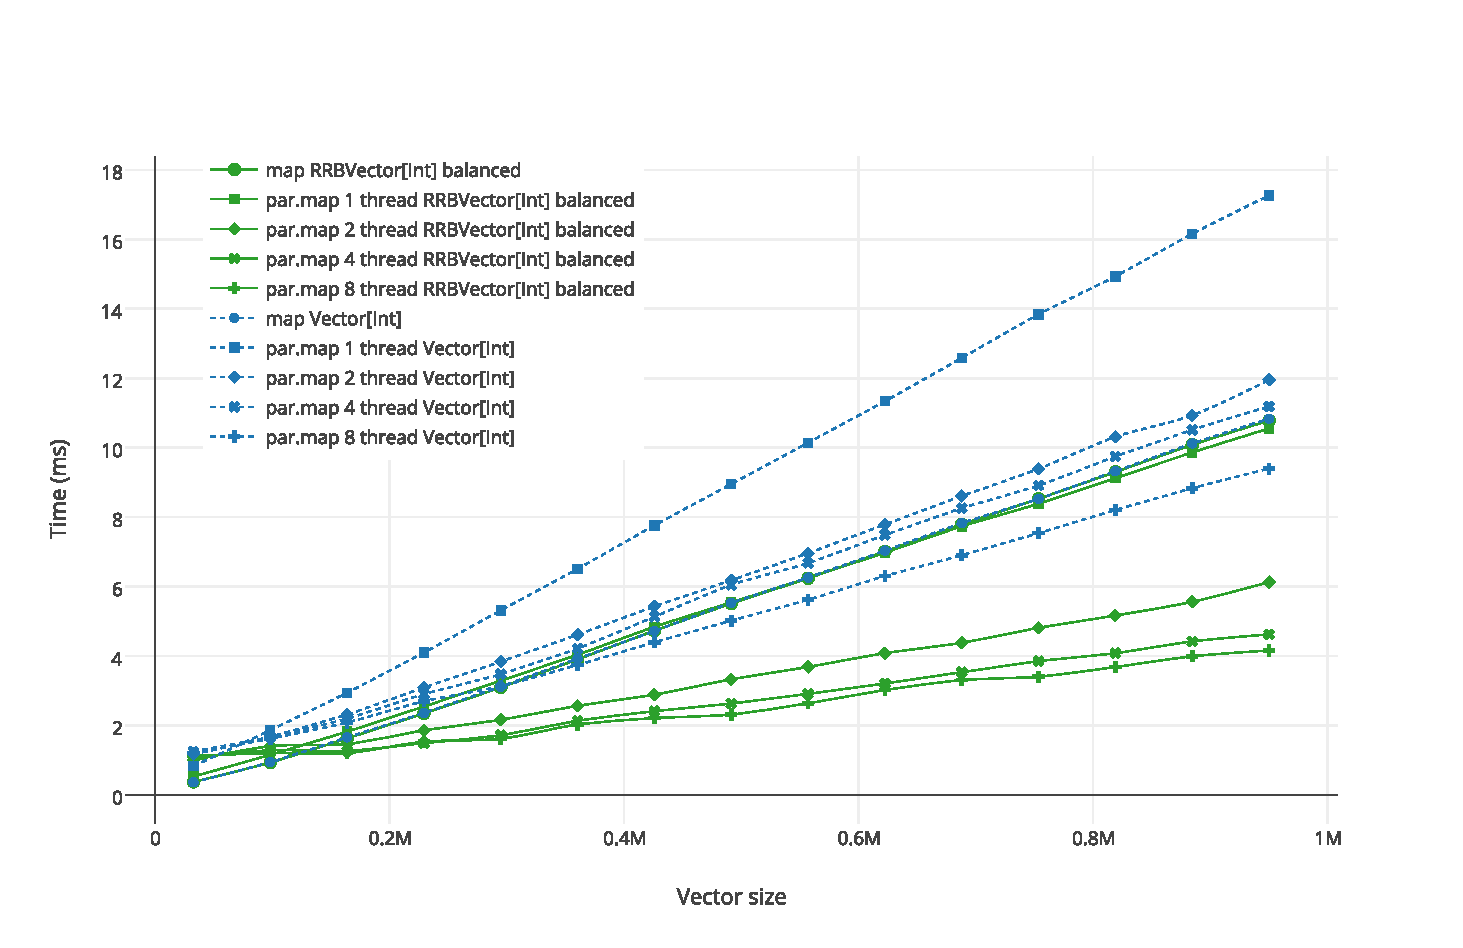
\includegraphics[width=\textwidth]{Benchmarks/Parmap_balanced.pdf}
  \caption{Benchmark on map and parallel map using the function (\textsc{x=>x}) to show the difference time used in the framework. This time represents the time spent in the splitters and combiners of the parallel collection (iterator and builder for the sequential version).}
  \label{ParallelBenchmarks}
\end{figure}

The current parallel \texttt{Vector} (that uses RB-Trees) results show that with 1, 2 and 4 threads the performance of the operation is worse. With 8 threads it becomes a little bit faster. This is what we expected, due to the lazy concatenation at the end of the combination of results. But, it show that this parallel collection is useless in practice.

When using the RRB-Vectors parallel, the parallelism is evident. With two threads the performance improvement is of almost 2X, then it tends to go towards 2.5X. This is the type of parallelism behaviour that is expected (see Amdahl's law\cite{Rodgers:1985:IMS:327010.327215}). Even the case on thread pool of one thread is a bit faster than the normal sequential one. 
\FloatBarrier

Figure \ref{ParallelUnbalancedBenchmarks} shows how unbalanced parallel vector behave. There is a slight loss in performance when they are unbalanced. But, this operations will create a balanced vector and therefore this small overhead can be amortized over the next operations.

\begin{figure}[h!]
  \centering
  \includegraphics[width=0.49\textwidth]{Benchmarks/parmap_unbalanced_1.pdf}
  \includegraphics[width=0.49\textwidth]{Benchmarks/parmap_unbalanced_2.pdf}
  \includegraphics[width=0.49\textwidth]{Benchmarks/parmap_unbalanced_4.pdf}
  \includegraphics[width=0.49\textwidth]{Benchmarks/parmap_unbalanced_8.pdf}
  \caption{Benchmark on map and parallel map using the function (\textsc{x=>x}) to show the difference time used in the framework. This time represents the time spent in the splitters and combiners of the parallel collection.}
  \label{ParallelUnbalancedBenchmarks}
\end{figure}

\FloatBarrier

%-----------------------------------
%	SUBSECTION Memory footprint
%-----------------------------------
\subsection{Memory footprint}
% describe the benchmark function
This is not really a benchmark, it is rather the characterization of the memory footprint of the vector that where used as input in the benchmarks. The aim of this is to show that even with the additional sizes of the unbalanced nodes and additional fields, the vectors size in memory is almost the same. 

% compare expectation with results
% explain the upper bound
% explain apparently incoherent results
Figure \ref{MemoryFootprints} shows that even for an extremely unbalanced RRB-Vector the increase in size is negligible. Fact for balanced ones it is even possible to have a smaller footprint (a few bytes) caused by the truncation of the last branch. 

\begin{figure}[h!]
  \centering
  \includegraphics[width=\textwidth]{Benchmarks/Memory_3.pdf}
  \caption{Memory Footprint for different vectors.}
  \label{MemoryFootprints}
\end{figure}

\FloatBarrier

Figure \ref{MemoryBlocksFootprints} shows the amount of space that could be saved by increasing the size of the block. The difference is not significant and as such the memory footprint is not a reason to change the size of blocks.

\begin{figure}[h!]
  \centering
  \includegraphics[width=\textwidth]{Benchmarks/Memory_blocks.pdf}
  \caption{Memory Footprint for different block sizes.}
  \label{MemoryBlocksFootprints}
\end{figure}

\FloatBarrier


I% Chapter Template

\chapter{Testing} % Main chapter title

\label{Testing} % Change X to a consecutive number; for referencing this chapter elsewhere, use \ref{ChapterX}

\lhead{Testing. \emph{Testing}} % Change X to a consecutive number; this is for the header on each page - perhaps a shortened title

%----------------------------------------------------------------------------------------
%	SECTION Teststing correctness
%----------------------------------------------------------------------------------------

%-----------------------------------
%	SUBSECTION Unit Tests
%-----------------------------------
\section{Black Box Testing}
% black box testing
% types of vector tested (balanced and different unbalanced vectors)
% pseudorandom set of differently unbalanced vectors
% comparing results of operations with other collections like lists
% use of tests suit on old Vector to check that tests are correct and coherent 
Tests on vector where done using the Scala Test framework. The test suite covers all core operations and some of the ones that are implemented in \texttt{IndexedSeq}. It also covers iterators, builders and parallel versions. Operations on \texttt{IndexedSeq} are crossed checked with other existing implementations.

The same test suite is used on the current \texttt{Vector} and on \texttt{RRBVector}. This way the test suite is also checked against the expected results from the current implementation. The test suite on \texttt{RRBVector} is executed on several sizes of vectors, with perfectly balanced vectors and several pseudo randomly unbalanced vectors. Each time a bug was identified, the test where extended to include the case where it failed.

These tests where usually executed in combination with the white box tests. This way test have a larger coverage and will fail at the moment where the bug first appeared. 

%-----------------------------------
%	SUBSECTION Invariant Assertions
%-----------------------------------
\section{White Box Testing}
\label{InvariantAssertions}
% white box testing with assertions
% explain how the invariants of the whole rrb-tree can be checked using assertions
% list and describe assertions used
White box testing is done using a set of heavy assertions on the invariants of the vector\footnote{This is implemented in the private method \texttt{assertVectorInvariant} of \texttt{RRBVector}.}. They test that the coherence of the three structure and the fields of vector. This test is done after the creation of any new vector object and after any canonicalization operation (see \ref{VectorCanonicalization}). This covers all the cases as no mutation is done in between of after those operations (assuming a non concurrent context). 

The vector invariant is divided into canonical and transient, where both test the same characteristics with some differences on the focused branch. The invariant includes tests on the bounds of \texttt{depth}, \texttt{endIndex}, \texttt{focus}, \texttt{focusStart}, \texttt{focusEnd}. It traverses the whole tree structure checking the structure of each node and crosschecking sizes (from \texttt{sizes} array and expected \texttt{endIndex}). For canonical states it checks the the branch in the displays is coherent with the tree an \texttt{focus}. For transient state it checks that the focused branch is unliked (or null). 

The current implementation of RRB-Vector has a static \text{Boolean} field to turn them on and off. When they are of they are dead code eliminated at compilation time. This feature must be disabled when in production due to its high overhead on operations. To protect the benchmark, they fail with an exception if it's enabled. The generated implementation (see \ref{ImplementationGenerators}) just create two different implementations, one without the assertions and one with them.


 
I% Chapter Template

\chapter{Related and Future Work} % Main chapter title

\label{RelatedWork} % Change X to a consecutive number; for referencing this chapter elsewhere, use \ref{ChapterX}

\lhead{\emph{Related and Future Work}} % Change X to a consecutive number; this is for the header on each page - perhaps a shortened title

%----------------------------------------------------------------------------------------
%	SECTION Related Work
%----------------------------------------------------------------------------------------
\section{Related Work}

List of related subjects:
\begin{itemize}
  \item RRB Trees and Vectors \cite{RRBTrees, lorange2014rrb, cormen2001introduction}
  \item Scala \cite{odersky2008programming,36605}
  \item Scala Collection \cite{ 1979992642, Oliveira:2010:TCO:1869459.1869489, EPFL-REPORT-200245}
  \item Scala Parallel Collection \cite{collect11,Lea:2000:JFF:337449.337465, 6264/THESES, Prokopec:2014aa}
  \item Functional data structures and semi-mutable data structures and related data structures \cite{Okasaki:1998:PFD:280586,DBLP:journals/jfp/HinzeP06, Driscoll:1989:MDS:64313.64317,4637966, Bayer:1970:OML:1734663.1734671, SPE:SPE4380251203, Bagwell01idealhash}
  \item Paper: Improving RRB-Tree Performance through Transience \cite{lorange2014rrb}
  \item Performance and Code specialization \cite{5456/THESES, Chafi:2011:DAH:1941553.1941561}
  \item JVM: Arrays, GC, JIT compiler \cite{Kotzmann:2008:DJH:1369396.1370017, Paleczny:2001:JHT:1267847.1267848, Wurthinger:2011:EGC:2048147.2048168}
  \item ScalaMeter \cite{Georges:2007:SRJ:1297027.1297033,scalameter}
  \item Scala Test \cite{scalatest}
  \item Scala Reflection and Quasiquotes \cite{EPFL-CONF-186844, quasiquotes}
  \item Type specialization and Miniboxing \cite{Ureche:2013:MIS:2509136.2509537, Ureche:2014:LDL:2660193.2660197, Stucki:2013:BIS:2489837.2489847, 4820/THESES, EPFL-REPORT-200245}
  \item Fusion \cite{Coutts:2007:SFL:1291151.1291199, scalablitz15}
\end{itemize}

\color{red} TODO: Cite references \color{black}

\paragraph{Paper: \emph{RRB-Trees: Efficient Immutable Vectors}}
\color{red} TODO \color{black}

\paragraph{Paper: \emph{Improving RRB-Tree Performance through Transience}}

% Describe the improvements proposed with transient mutable states

% Describe fundamental difference between this transience and the display one.

\color{red} TODO \color{black}



%----------------------------------------------------------------------------------------
%	SECTION Related Work
%----------------------------------------------------------------------------------------
\section{Future Work}

\paragraph{Mesure unbalance}
% find a good measurement of unbalancess to characterise vectors
% characterize vectors on real world programs
One analysis that was left out of the scope of this project was the characterization of the vectors unbalance. There is currently no way to quantitatively measure the unbalance of on the tree node. Some ideas for this are: number of unbalanced nodes, number of balanced subtrees, average height of balanced subtrees, ... 

Once this measurement exists it would be possible would be possible to conduct a real world application characterisation of fe vectors. And see how common the unbalanced vectors are and if they are only slightly unbalanced or extremely unbalanced. From this it would be possible to give a true expected performance for the cases where the performances differ.

\paragraph{Simplify Code}
% use macros to define core operations of the vector to simplify expanded code (half of the work is already done on the generators)
It should be possible to simplify and reduce the amount of code of the Scala implementation of vector using Scala Macros\footnote{Or Scala Meta in the future} to expand and optimize the code that was done manually. This was partially done on the vector implementation generators (see \ref{ImplementationGenerators}), where some key abstractions generate most of the expansions. This is a good basis to write such macros.

% fallthroug switch
Another way to simplify the code would involve the creation of a new abstraction that would compile down to bytecode \texttt{tableswitch} instructions with fallthroughs. A switch with no \texttt{break}s should be enough\footnote{Look at \texttt{copyDisplays} function in the code, the \texttt{if/else} expressions could be replaced by a single \texttt{switch} statement.}. This could help a bit with performance.

\paragraph{Formalization}
% formal proof of correctness of relaxed operations
% formal proof of correctness of canonicalisation
There is still the need for formal proof on some operations. Mainly for the optimized implementations of the relaxed relaxed operations. The canonicalization operation of the vector also needs a formal proof and may be a interesting study case for immutable data structures with simple internal mutation schemes.

%\paragraph{String concatenation} 
%Explore the possibility of improving string concatenation using RRB vector. It would probably not be a good idea to use a vector of characters as a string due to overhead on memory an access time due to boxing of characters (this is speculation). Rather try to represent the result of string concatenations in a vector of strings. If a wrapper is used, it could use the same technique as the canonicalization to generate the actual string if needed and drop the vector. Compare performance with other string representation (like ropes \cite{SPE:SPE4380251203}).

 
I% Chapter Template

\chapter{Conclusions} % Main chapter title

\label{Conclusions} % Change X to a consecutive number; for referencing this chapter elsewhere, use \ref{ChapterX}

\lhead{\emph{Conclusions}} % Change X to a consecutive number; this is for the header on each page - perhaps a shortened title

%----------------------------------------------------------------------------------------
%	CONCLUSIONS
%----------------------------------------------------------------------------------------

% implemented
%% without loosing the optimization (effects reduced in some cases)

% performance 
%% in most cases there is no loss
%% when there is loss, the performance is still bounded by a constant

% showed that branching of 32 is still the best option

% showed improvement on parallel vectors





\color{red} TODO \color{black}

 

%----------------------------------------------------------------------------------------
%	THESIS CONTENT - APPENDICES
%----------------------------------------------------------------------------------------

%\addtocontents{toc}{\vspace{2em}} % Add a gap in the Contents, for aesthetics

%\appendix % Cue to tell LaTeX that the following 'chapters' are Appendices

% Include the appendices of the thesis as separate files from the Appendices folder
% Uncomment the lines as you write the Appendices

%\input{Appendices/AppendixA}
%\input{Appendices/AppendixB}
%\input{Appendices/AppendixC}

%\addtocontents{toc}{\vspace{2em}} % Add a gap in the Contents, for aesthetics

%\backmatter

%----------------------------------------------------------------------------------------
%	BIBLIOGRAPHY
%----------------------------------------------------------------------------------------

\label{Bibliography}

\lhead{\emph{Bibliography}} % Change the page header to say "Bibliography"

\bibliographystyle{unsrtnat} % Use the "unsrtnat" BibTeX style for formatting the Bibliography

\bibliography{Bibliography} % The references (bibliography) information are stored in the file named "Bibliography.bib"

\end{document}